\documentclass{report} % Pagina con solo logo, titolo, indice e altre informazioni

\usepackage[utf8]{inputenc}
\usepackage[italian]{babel}

\usepackage[margin=3.0cm]{geometry} %Per avere un margine di 3.0 cm
\usepackage{multirow} %Per poter inserire celle multiriga
\usepackage{graphicx} % Utilizzato per mostrare immagini (\includegraphics)
\usepackage[colorlinks=true, allcolors=black]{hyperref} %Per avere link

%Per controllare la larghezza delle colonne nelle tabelle
\usepackage{array} 
    \newcolumntype{L}[1]{>{\raggedright\let\newline\\\arraybackslash\hspace{0pt}}m{#1}}
    \newcolumntype{C}[1]{>{\centering\let\newline\\\arraybackslash\hspace{0pt}}m{#1}}
    \newcolumntype{R}[1]{>{\raggedleft\let\newline\\\arraybackslash\hspace{0pt}}m{#1}}

%Per avere tabelle su più pagine
\usepackage{longtable}
\usepackage{multirow}

%Per controllare la visualizzazione dei capitoli
\usepackage{titlesec}
    \titleformat{\chapter}[display]{\normalfont}{\LARGE\scshape Capitolo \thechapter}{0.5cm}{\huge\bfseries}
    \titlespacing{\chapter}{0cm}{-0.7cm}{1.4cm} 
    
\setlength{\parindent}{0.7cm} %Per impostare l'interspazio di tutti i paragrafi a 0.7 cm

\setcounter{chapter}{-1} %Per far iniziare la numerazione dei capitoli da 0

%Info documento
\title{DietiDeals24}
\author{
    Scisciola Simone
    \and
    Carandente Ilaria Giuseppina
    \and
    Lucchese Andrea
}
\date{Anno Accademico 2023-2024}

%Inizio documento
\begin{document}
    \begin{titlepage} %Per non far comparire il numero di pagina in basso
    
        \begin{figure}[htbp!]
            \begin{center}
                \includegraphics[width=.30\textwidth]{Immagini/Logo/FedericoII.png}
            \end{center}
        \end{figure}
        
        \begin{center}
        
            \textbf{\LARGE DietiDeals24}
        
            \vspace{3\baselineskip}
            
            {\LARGE Università degli Studi di Napoli Federico II}         
            \vspace{1\baselineskip}
            
            {\large Scuola Politecnica e delle Scienze di Base \\
            Dipartimento di Ingegneria Elettrica e delle Tecnologie dell’Informazione \\
            Corso di Laurea in Informatica}
            \vspace{1\baselineskip}
            
            Anno Accademico 2023-2024
            \vspace{8\baselineskip}


            
            {\large \bfseries Scisciola Simone} \\
            N86004025
    	  \vspace{1\baselineskip}
    
            {\large \bfseries Lucchese Andrea} \\
            N86004112
    	  \vspace{1\baselineskip}
    
            {\large \bfseries Carandente Ilaria Giuseppina} \\
            N86004269
            \vspace{10\baselineskip}


    
    	  {\large \today}
       
        \end{center}
    \end{titlepage}

\newpage

    \tableofcontents
    
    \include{Argomenti/Capitolo0/Traccia}
    \chapter{Glossario}
    \section{Obiettivo}
        In questa sezione sono definiti i vocaboli meno comuni utilizzati all'interno della documentazione.

    \section{Glossario}
        \begin{tabular}{|C{3.5cm}|L{11.2cm}|}
            \hline
            \multicolumn{1}{|c|}{\cellcolor{head}\textbf{Vocabolo}} & \multicolumn{1}{c|}{\cellcolor{head}\textbf{Definizione}}\\
            \hline
                Stakeholders &
                Insieme dei soggetti che hanno un interesse nei confronti di un'organizzazione e che con il loro comportamento possono influenzarne l'attività. Nel caso dell'ingegneria del software, tutti gli individui interessati alla messa in opera del sistema. \\
            \hline
                Requirement Elicitation &
                Raccolta dei requisiti. \\
            \hline
                Requirement Analysis &
                Analisi dei requisiti. \\
            \hline
                Requirement Specification &
                Specifica dei requisiti. \\
            \hline
                System Design &
                Progettazione del sistema. \\
            \hline
                Object Design &
                Progettazione orientata agli oggetti. \\
            \hline
                Utente loggato &
                Utente che ha effettuato il login, ovvero l'accesso al proprio account. \\
            \hline
                Utente target &
                Utente "tipico" che utilizzerà l'applicativo, individuato a seguito di uno studio demografico. \\
            \hline
                Use Case Diagram &
                Diagramma dei casi d'uso. \\
            \hline
                Class Diagram &
                Diagramma delle classi. \\
            \hline
                Sequence Diagram &
                Diagramma di sequenza. \\
            \hline
                Statechart Diagram &
                Diagramma degli stati. \\
            \hline
                NRU &
                Not Registered User (utente non registrato). \\
            \hline
                RU &
                Registered User (utente registrato). \\
            \hline
                USR &
                User (utente, non registrato o registrato). \\
            \hline
                BUY &
                Buyer (compratore). \\
            \hline
                SEL &
                Seller (venditore). \\
            \hline
                SYS &
                System (sistema). \\
            \hline
        \end{tabular}
    %PDF DI RIFERIMENTO: 03_Requirement Engineering.pdf

\chapter{Requirement Elicitation}
    \section{Obiettivo}
        A seguito di una intervista agli stakeholders per carpire informazioni sul dominio del problema, nonché le funzionalità e le qualità che il software debba possedere per risultare conforme ai bisogni dell'utente, si elencano di seguito tutti i requisiti di sistema individuati:
    \section{Introduzione al sistema} %Requisiti sistema. 1 pagina
% 1
        \begin{itemize}
            \item L'utente che non ha effettuato l'accesso può registrarsi con email correttamente formattata e password.
            \item Il sistema controlla che l'email abbia il formato corretto (ovvero sia del tipo x+@y+.z+) e che la password sia sicura (ovvero sia lunga almeno 8 caratteri e contenga, nel complesso, almeno una lettera maiuscola [A-Z], un numero [0-9] e un carattere speciale [!@\#\$\%\^{}\&*])
            \item L'utente che non ha effettuato l'accesso può registrarsi con altri account già esistenti come Google, Facebook, GitHub e X.
            \item L'utente che non ha effettuato l'accesso può selezionare se il suo nuovo account è di tipo compratore o venditore.
            \item L'utente che non ha effettuato l'accesso può creare uno e un solo account di tipo compratore con la stessa email.
            \item L'utente che non ha effettuato l'accesso può creare uno e un solo account di tipo venditore con la stessa email.
            \item L'utente che non ha effettuato l'accesso può creare un profilo condiviso tra l'account venditore e l'account compratore con la stessa email. La creazione del profilo avviene subito dopo la fase di registrazione account.
            \item L'utente che non ha effettuato l'accesso può accedere a un account con l'email e password utilizzati nella registrazione.
            \item L'utente che non ha effettuato l'accesso può accedere con altri account già esistenti come Google, Facebook, GitHub e X.
            \item L'utente che ha effettuato l'accesso può visualizzare il suo profilo.
            \item L'utente che ha effettuato l'accesso può modificare i dati sul suo profilo, come biografia, link al proprio sito, link social e area geografica.
        \end{itemize}
% 2
        \begin{itemize}
            \item Il venditore può creare aste di vendita di un prodotto/servizio. L'asta risulterà attiva (cioè sarà possibile presentare offerte) fin da subito.
            \item Il venditore può selezionare il tipo di asta da creare. L'asta può essere di tipo "a tempo fisso" o "silenziosa".
            \item Il venditore di un'asta di qualsiasi tipo può inserire, al momento della creazione dell'asta, una data e ora di scadenza, un titolo, una descrizione, una categoria e opzionalmente una o più fotografie per l'asta da lui creata.
            \item Il venditore di un'asta di qualsiasi tipo può modificare la data e ora di scadenza, il titolo, la descrizione, la categoria e le fotografie (se aggiunte) per l'asta da lui creata.
            \item Il compratore può presentare offerte per le aste correntemente attive e gestite da venditori.
        \end{itemize}
% 3
        \begin{itemize}
            \item L'utente (sia che abbia effettuato l'accesso, sia che non l'abbia effettuato) può ricercare le aste attraverso parole chiave.
            \item L'utente (sia che abbia effettuato l'accesso, sia che non l'abbia effettuato) può ricercare le aste sulla base della categoria.
            \item L'utente (sia che abbia effettuato l'accesso, sia che non l'abbia effettuato) può visualizzare i dettagli di un'asta.
            \item L'utente (sia che abbia effettuato l'accesso, sia che non l'abbia effettuato) può visualizzare il profilo del proprietario dell'asta.
            \item L'utente (sia che abbia effettuato l'accesso, sia che non l'abbia effettuato) può visualizzare le aste attive.
            \item L'utente che ha effettuato l'accesso può visualizzare le aste che ha creato.
            \item L'utente che ha effettuato l'accesso può eliminare le aste che ha creato.
            \item L'utente che ha effettuato l'accesso può visualizzare le aste a cui ha partecipato.
            \item L'utente che ha effettuato l'accesso può visualizzare l'elenco delle offerte proposte alle aste da lui create.
        \end{itemize}
% 4
        \begin{itemize}
            \item Il venditore di un asta di tipo "a tempo fisso" può stabilire, al momento della creazione dell'asta, una soglia minima segreta per l'asta da lui creata (mai visibile ad altri utenti al di fuori del creatore dell'asta e deve essere un valore maggiore o uguale a 0).
            \item L'utente (sia che abbia effettuato l'accesso, sia che non l'abbia effettuato) può visualizzare l'attuale offerta più alta dell'asta di tipo "a tempo fisso".
            \item Il sistema assegna la vincita al compratore di un asta di tipo "a tempo fisso" che ha offerto la somma più alta entro la data e ora di scadenza dell'asta.
            \item Il sistema dichiara l'asta fallita se nessun compratore di un asta di tipo "a tempo fisso" ha offerto una somma più alta della soglia minima entro la data e ora di scadenza dell'asta.
            \item Il sistema dichiara l'asta fallita se non è stata avanzata alcuna offerta da parte di un compratore di un'asta di tipo "a tempo fisso" entro la data e ora di scadenza dell'asta.
            \item L'utente che ha effettuato l'accesso può visualizzare le proprie notifiche.
            \item Il sistema invia una notifica di chiusura dell'asta a tutti i partecipanti dell'asta di tipo "a tempo fisso" (ovvero il venditore e tutti i compratori che hanno offerto almeno una volta una somma di denaro) entro 10 secondi dalla data e ora di scadenza dell'asta.
        \end{itemize}
% 7
        \begin{itemize}
            \item Il sistema mostra l'offerta di un'asta di tipo "silenziosa" solo al venditore di tale asta e a colui che ha proposto l'offerta.
            \item Il venditore di un'asta di tipo "silenziosa" può accettare una e una sola offerta, inviata tra le offerte non ancora rifiutate dell'asta di tipo "silenziosa" da lui creata.
            \item Il venditore di un'asta di tipo "silenziosa" può rifiutare le singole offerte ricevute all'asta di tipo "silenziosa" da lui creata.
            \item Il sistema assegna la vincita dell'asta al compratore di un'asta di tipo "silenziosa" la cui offerta è stata accettata dal venditore dell'asta di tipo "silenziosa".
            \item Il sistema dichiara l'asta fallita se il venditore di un'asta di tipo "silenziosa" non ha accettato alcuna offerta entro la data e ora di scadenza dell'asta.
            \item Il sistema dichiara l'asta fallita se non è stata avanzata alcuna offerta da parte di un compratore di un'asta di tipo "silenziosa" entro la data e ora di scadenza dell'asta.
            \item Il sistema invia una notifica di proposta offerta al venditore dell'asta di tipo "silenziosa" che ha ricevuto una nuova offerta alla propria asta.
            \item Il sistema invia una notifica di chiusura dell'asta a tutti i partecipanti dell'asta di tipo "silenziosa" (ovvero a tutti i compratori che hanno offerto almeno una volta una somma di denaro) entro 10 secondi dal momento in cui è stata accettata un'offerta. Tale notifica indicherà se la propria offerta è stata accettata o rifiutata.
            \item Il sistema invia una notifica di rifiuto dell'offerta al partecipante dell'asta di tipo "silenziosa" la cui offerta è stata rifiutata dal venditore dell'asta.
        \end{itemize}
% 8
        \begin{itemize}            
            \item Il compratore può creare un'asta di tipo "inversa".
            \item Il compratore di un'asta di tipo "inversa" può inserire, al momento della creazione dell'asta, una data e ora di scadenza, un titolo, una descrizione, una categoria, un prezzo di partenza che è disposto a pagare e opzionalmente una o più fotografie per l'asta da lui creata.
            \item Il compratore di un'asta di tipo "inversa" può modificare la data e ora di scadenza, il titolo, la descrizione, la categoria e le fotografie (se aggiunte) per l'asta da lui creata.
            \item Il venditore in grado di fornire quel particolare prodotto/servizio può presentare offerte per le aste di tipo "inversa" entro la data e ora di scadenza dell'asta. Tale offerta è una somma in euro minore rispetto alla somma più bassa attualmente raggiunta (tale valore deve essere maggiore o uguale a 0).
            \item Il sistema assegna la vincita dell'asta di tipo "inversa" al venditore che ha offerto la somma più bassa al sopraggiungere della data e ora di scadenza dell'asta a cui ha partecipato.
            \item Il sistema dichiara l'asta di tipo "inversa" fallita se non è stata avanzata alcuna offerta da parte di un venditore entro la data e ora di scadenza dell'asta.
            \item Il sistema invia una notifica di chiusura dell'asta a tutti i partecipanti dell'asta di tipo "inversa" (ovvero il compratore e tutti i venditori che hanno offerto almeno una volta una somma di denaro) entro 10 secondi dalla data e ora di scadenza dell'asta.
        \end{itemize}
    %PDF DI RIFERIMENTO: 03_Requirement Engineering.pdf, Personas.pdf

\chapter{Requirement Analysis}
    \section{Obiettivo}
        Le informazioni ottenute attraverso la raccolta sono state organizzate attraverso l'uso di diagrammi ad alto livello, quali diagramma UML dei casi d'uso, tabelle di Cockburn e mock-up. \\
        Sono stati anche individuati gli utenti target del sistema, nonché sono stati effettuati test di usabilità a priori sui mock-up dell'interfaccia utente.

    \section{Use Case Diagram}
        Il diagramma dei casi d'uso indica per ciascun attore (utente che utilizzerà il sistema) quali sono le funzionalità alle quali egli potrà accedere.
        %Use Case Diagram costruito con StarUML
        \begin{figure}[htbp!]
            \centering
                \includegraphics[width=0.378\linewidth]{Immagini/Diagrammi/UseCaseDiagram.pdf}
            \caption{Use Case Diagram}
            \label{fig:Use Case Diagram}
        \end{figure}
    
    \section{Utenti target}
        L'individuazione di utenti target risulta cruciale per sviluppare un applicativo che possa essere indirizzato ad una specifica demografica. \\
        In particolare, permette di comprendere quali sono i bisogni delle diverse tipologie di utenti, rendendo semplici le operazioni che hanno bisogno di effettuare più spesso ciascuno di loro e risolvere le frustrazioni che essi possono riscontrare nei confronti di applicativi già esistenti. \\
        Lo studio avviene attraverso la creazione di mock-up definiti "personas". Abbiamo indiviuato in totale sei gruppi di utenti, dei quali i più prominenti sono quelli rappresentati da Maria Lombardo (persona primaria) e Luca Serra (persona secondaria).
        
        \begin{figure}[!htb]
           \begin{minipage}{0.48\textwidth}
                \centering
             \includegraphics[width=.7\linewidth]{Immagini/Personas/Maria Lombardo.pdf}
             \caption{Maria Lombardo}\label{Fig:Maria Lombardo}
           \end{minipage}\hfill
           \begin{minipage}{0.48\textwidth}
                \centering
             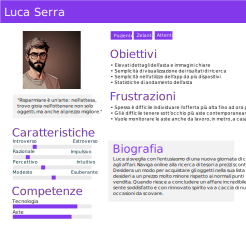
\includegraphics[width=.7\linewidth]{Immagini/Personas/Luca Serra.pdf}
             \caption{Luca Serra}\label{Fig:Luca Serra}
           \end{minipage}
        \end{figure}

        \begin{figure}[!htb]
           \begin{minipage}{0.48\textwidth}
                \centering
             \includegraphics[width=.7\linewidth]{Immagini/Personas/Marco Rossi.pdf}
             \caption{Marco Rossi}\label{Fig:Marco Rossi}
           \end{minipage}\hfill
           \begin{minipage}{0.48\textwidth}
                \centering
             \includegraphics[width=.7\linewidth]{Immagini/Personas/Martina Silvestri.pdf}
             \caption{Martina Silvestri}\label{Fig:Martina Silvestri}
           \end{minipage}
        \end{figure}

        \clearpage
        
        \begin{figure}[!htb]
           \begin{minipage}{0.48\textwidth}
                \centering
             \includegraphics[width=.7\linewidth]{Immagini/Personas/Matteo Luongo.pdf}
             \caption{Matteo Luongo}\label{Fig:Matteo Luongo}
           \end{minipage}\hfill
           \begin{minipage}{0.48\textwidth}
                \centering
             \includegraphics[width=.7\linewidth]{Immagini/Personas/Arturo Campobello.pdf}
             \caption{Arturo Campobello}\label{Fig:Arturo Campobello}
           \end{minipage}
        \end{figure}

    \newpage
    
    \section{Tabelle di Cockburn e Mock-up}
    La realizzazione dell'interfaccia è stata eseguita attraverso il software di prototipazione Figma (il link al mock-up è visualizzabile \href{https://www.figma.com/file/kieERzm8U3jsHALXk4IjKS/Mockup?type=design&node-id=0%3A1&mode=design&t=CAyNdczd5giYLJ1j-1}{\underline{qui}}). \\
    Il software ha consentito di individuare l'assetto generale dell'interfaccia utente per l'esecuzione di ogni caso d'uso individuato, nonché indicare le trasformazioni dell'interfaccia stessa in caso di errori del sistema.\\
    Basandosi sull'interfaccia realizzata, è stata effettuata la stesura delle tabelle di Cockburn di due casi d'uso significativi. \\
    Lo scopo delle tabelle è quello di presentare in maniera sequenziale come giungere all'esecuzione di un caso d'uso interagendo con l'interfaccia utente. \\
    Sono stati evidenziati anche possibili metodi alternativi per raggiungere lo stesso scopo o errori che potrebbero sorgere.
        \subsection{Crea un’asta inversa}
            \begin{longtable}{|C{3.0cm}|C{1.3cm}|L{5.2cm}|L{5.2cm}|}
                \hline
                    \textbf{USE CASE \#1} &
                    \multicolumn{3}{|l|}{\textbf{Crea un’asta inversa}}\\
                \hline
                    Goal in Context &
                    \multicolumn{3}{|l|}{L'utente di tipo "compratore" vuole creare un'asta inversa.}\\
                \hline
                    Preconditions &
                    \multicolumn{3}{|l|}{L'utente ha effettuato l'accesso con un account di tipo "compratore".}\\
                \hline
                    Success End Condition &
                    \multicolumn{3}{|l|}{L'utente di tipo "compratore" ha correttamente creato un'asta "inversa"}\\
                \hline
                    \multirow[|c|]{32}{*}{DESCRIPTION} 
                    & \textbf{Step n°}
                    & \textbf{Compratore}
                    & \textbf{Sistema}\\
                \cline{2-4}
                        & 1
                        & Preme bottone "Crea asta" su mock-up C1 (Figura 3.8)
                        & \\
                \cline{2-4}
                        & 2
                        & 
                        & Mostra mock-up P0 (Figura ???) con testo "Seleziona tipo di asta" dove è possibile scegliere il tipo di asta da creare.\\
                \cline{2-4}
                        & 3
                        & Seleziona "Inversa" e clicca "Conferma" sul mock-up P0 (Figura ???)
                        & \\
                \cline{2-4}
                        & 4
                        & 
                        & Mostra mock-up C4 (Figura 3.9) con tutte le informazioni dell'asta inversa da poter inserire.\\
                \cline{2-4}
                        & 5
                        & Preme sul campo di input "Data di scadenza"
                        & \\
                \cline{2-4}
                        & 6
                        & 
                        & Mostra il pannello di selezione della data da calendario\\
                \cline{2-4}
                        & 7
                        & Seleziona la data
                        & \\
                \cline{2-4}
                        & 8
                        & Clicca su OK
                        & \\
                \cline{2-4}
                        & 9
                        & 
                        & Scrive la data selezionata nel campo di input "Data di scadenza"\\
                \cline{2-4}
                        & 10
                        & Preme sul campo di input "Ora di scadenza"
                        & \\
                \cline{2-4}
                        & 11
                        & 
                        & Mostra il pannello di selezione dell'ora\\
                \cline{2-4}
                        & 12
                        & Seleziona l'ora
                        & \\
                \cline{2-4}
                        & 13
                        & Clicca su OK
                        & \\
                \cline{2-4}
                        & 14
                        & 
                        & Scrive l'ora selezionata nel campo di input "Ora di scadenza"\\
                \cline{2-4}
                        & 15
                        & Preme sul campo di input "Prezzo di partenza"
                        & \\
                \cline{2-4}
                        & 16
                        &
                        & Mostra il tastierino numerico \\
                \cline{2-4}
                        & 17
                        & Inserisce il prezzo di partenza
                        & \\
                \cline{2-4}
                        & 18
                        & Preme sul campo di input "Nome prodotto"
                        & \\
                \cline{2-4}
                        & 19
                        &
                        & Mostra la tastiera \\
                \cline{2-4}
                        & 20
                        & Inserisce il nome del prodotto oggetto dell'asta
                        & \\
                \cline{2-4}
                        & 21
                        & Preme sul campo di input "Categoria"
                        & \\
                \cline{2-4}
                        & 22
                        &
                        & Mostra il menù a tendina con le diverse categorie tra cui scegliere \\
                \cline{2-4}
                        & 23
                        & Seleziona la categoria
                        & \\
                \cline{2-4}
                        & 24
                        & 
                        & Scrive la categoria scelta nel campo di input "Categoria"\\
                \cline{2-4}
                        & 25
                        & Preme sul campo di input "Descrizione"
                        & \\
                \cline{2-4}
                        & 26
                        &
                        & Mostra la tastiera \\
                \cline{2-4}
                        & 27
                        & Inserisce la descrizione del prodotto oggetto dell'asta
                        & \\
                \cline{2-4}
                        & 28
                        & Preme sul pulsante "Crea"
                        & \\
                \cline{2-4}
                        & 29
                        & 
                        & Mostra mock-up P20 (Figura 3.10, Pop-up di successo)\\
                \cline{2-4}
                        & 30
                        & Preme il pulsante X sul mock-up P20 (Figura 3.10)
                        & \\
                \cline{2-4}
                        & 31
                        & 
                        & Torna al mock-up C1 (Figura 3.8, Finestra Home)\\
                \hline
                    EXTENSIONS
                    & \textbf{Step n°} 
                    & \textbf{Compratore} 
                    & \textbf{Sistema}\\
                \hline
                    \multirow[|c|]{2}{*}{\shortstack[c]{Seleziona asta \\ diversa da quella \\ inversa}}
                        & 3.a
                        & Seleziona tipo di asta diversa da "Inversa" e clicca "Conferma" sul mock-up P0 (Figura ???)
                        & \\
                \cline{2-4}
                        & 4.a
                        & 
                        & Mostra mock-up di creazione asta relativo all'asta selezionata\\
                \hline
                    \multirow[|c|]{3}{*}{\shortstack[c]{Seleziona data \\  antecedente a \\quella odierna}}
                        & 9.b
                        & 
                        & Mostra mock-up P19 (Figura 3.11) con testo "Non puoi inserire una data antecedente a quella odierna!"\\
                \cline{2-4}
                        & 10.b
                        & Clicca su X sul mock-up P19 (Figura 3.11)
                        & \\
                \cline{2-4}
                        & 11.b
                        & 
                        & Continua da step 3 di main scenario\\
                \hline
                    \multirow[|c|]{3}{*}{\shortstack[c]{Seleziona data \\ odierna e ora \\ antecedente a \\quella attuale}}
                        & 14.c
                        & 
                        & Mostra mock-up P14 (Figura 3.12) con testo "Non puoi selezionare un’ora antecedente a quella attuale in data odierna!"\\
                \cline{2-4}
                        & 16.c
                        & Clicca su X sul mock-up P14 (Figura 3.12)
                        & \\
                \cline{2-4}
                        & 17.c
                        & 
                        & Continua da step 8 di main scenario\\
                \hline
                    \multirow[|c|]{3}{*}{\shortstack[c]{Seleziona prezzo di \\ partenza negativo}}
                        & 18.d
                        & 
                        & Mostra mock-up P10 (Figura 3.13) con testo "Non puoi inserire una somma di partenza minore di 0 €."\\
                \cline{2-4}
                        & 19.d
                        & Clicca su X sul mock-up P10 (Figura 3.13)
                        & \\
                \cline{2-4}
                        & 20.d
                        & 
                        & Continua da step 13 di main scenario\\
                \hline
                    \multirow[|c|]{1}{*}{\shortstack[c]{Alcuni campi \\ obbligatori non \\ compilati}}
                        & 29.e
                        & 
                        & Mostra mock-up E11 (Figura 3.14) dove vengono segnalati in rosso i campi obbligatori non compilati\\
                \cline{2-4}
                        & 30.e
                        & Riparte da step 3 di main scenario, saltando i campi di input già compilati
                        & \\
                \hline
                    \multirow[|c|]{4}{*}{\shortstack[c]{Esce dalla pagina \\ di creazione asta}}
                        & \textit{In qualunque passo del main scenario}
                        & Preme qualsiasi tasto di navigazione (della navbar in basso o tasto "indietro" del dispositivo)
                        & \\
                \cline{2-4}
                        & 
                        & 
                        & Mostra mock-up P6 (Figura 3.15) con testo "Se uscirai da questa schermata, i dati inseriti nei campi saranno cancellati. Vuoi proseguire?" \\
                \cline{2-4}
                        & 
                        & Clicca su Esci sul mock-up P6 (Figura 3.15)
                        & \\
                \cline{2-4}
                        & 
                        & 
                        & Mostra mock-up corrispondente al tasto cliccato\\
                \hline
                    SUBVARIATIONS
                    & \textbf{Step n°} 
                    & \textbf{Compratore} 
                    & \textbf{Sistema}\\
                \hline
                    \multirow[|c|]{5}{*}{\shortstack[c]{Inserisce immagine}}
                        & 18.s1
                        & Preme sul campo di input "Aggiungi immagine prodotto"
                        & \\
                \cline{2-4}
                        & 19.s1
                        & 
                        & Mostra il sistema per selezionare le immagini\\
                \cline{2-4}
                        & 20.s1
                        & Seleziona una o più immagini
                        & \\
                \cline{2-4}
                        & 21.s1
                        & Clicca su OK
                        & \\
                \cline{2-4}
                        & 22.s1
                        & 
                        & Continua da step 16 di main scenario\\
                \hline
            \end{longtable}

            \begin{figure}[!htb]
            \begin{minipage}{0.32\textwidth}
                \centering
                \includegraphics[width=.7\linewidth]{Immagini/Frames/Compratore/C1.pdf}
                \caption{Home compratore}
            \end{minipage}\hfill
            \begin{minipage}{0.32\textwidth}
                \centering
                \includegraphics[width=.7\linewidth]{Immagini/Frames/Compratore/C4.pdf}
                \caption{Crea asta compratore}
            \end{minipage}\hfill
            \begin{minipage}{0.32\textwidth}
                \centering
                \includegraphics[width=.7\linewidth]{Immagini/Frames/Popup/P20.pdf}
                \caption{Successo creazione asta}
            \end{minipage}\hfill
        \end{figure}
    
        \begin{figure}[!htb]
            \begin{minipage}{0.32\textwidth}
                \centering
                \includegraphics[width=.7\linewidth]{Immagini/Frames/Popup/P19.pdf}
                \caption{Errore data non valida}
            \end{minipage}\hfill
            \begin{minipage}{0.32\textwidth}
                \centering
                \includegraphics[width=.7\linewidth]{Immagini/Frames/Popup/P14.pdf}
                \caption{Errore ora non valida}
            \end{minipage}\hfill
            \begin{minipage}{0.32\textwidth}
                \centering
                \includegraphics[width=.7\linewidth]{Immagini/Frames/Popup/P10.pdf}
                \caption{Errore somma di partenza non valida}
            \end{minipage}\hfill
        \end{figure}
    
        \begin{figure}[!htb]
            \begin{minipage}{0.32\textwidth}
                \centering
                \includegraphics[width=.7\linewidth]{Immagini/Frames/Errori/E11.pdf}
                \caption{Errore campi obbligatori non compilati}
            \end{minipage}\hfill
            \begin{minipage}{0.32\textwidth}
                \centering
                \includegraphics[width=.7\linewidth]{Immagini/Frames/Popup/P6.pdf}
                \caption{Richiesta conferma uscita}
            \end{minipage}\hfill
        \end{figure}

        \clearpage
        
        \subsection{Accetta un'offerta ricevuta all'asta silenziosa}
            \begin{longtable}{|C{3.0cm}|C{1.3cm}|L{5.2cm}|L{5.2cm}|}
                \hline
                    \textbf{USE CASE \#2} &
                    \multicolumn{3}{|l|}{\textbf{Accetta un'offerta ricevuta all'asta silenziosa}}\\
                \hline
                    Goal in Context &
                    \multicolumn{3}{|l|}{\shortstack[l]{L'utente di tipo "venditore" vuole accettare un'offerta ricevuta in un'asta \\ "silenziosa" da lui creata}}\\
                \hline
                    Preconditions &
                    \multicolumn{3}{|l|}{\shortstack[l]{L'utente ha effettuato l'accesso con un account di tipo "venditore" e ha creato \\ un'asta "silenziosa"}}\\
                \hline
                    Success End Condition &
                    \multicolumn{3}{|l|}{\shortstack[l]{L'utente di tipo "venditore" ha correttamente accettato un'offerta di un'asta \\ "silenziosa" da lui creata}}\\
                \hline
                    \multirow[|c|]{11}{*}{DESCRIPTION} 
                    & \textbf{Step n°}
                    & \textbf{Venditore di asta silenziosa}
                    & \textbf{Sistema}\\
                \cline{2-4}
                        & 1
                        & Preme bottone "Profilo" su mock-up V1 (Figura 3.16)
                        & \\
                \cline{2-4}
                        & 2
                        & 
                        & Mostra mock-up V7 (Figura 3.17) con tutte le opzioni per utenti loggati.\\
                \cline{2-4}
                        & 3
                        & Preme sul bottone "Le mie aste create".
                        & \\
                \cline{2-4}
                        & 4
                        & 
                        & Mostra il mock-up V11 (Figura 3.18) con tutte le aste create dal venditore.\\
                \cline{2-4}
                        & 5
                        & Clicca sull'icona a forma di elenco dell'asta di cui si vogliono visualizzare le offerte ricevute.
                        & \\
                \cline{2-4}
                        & 6
                        & 
                        & Mostra mock-up V13 (Figura 3.19) con l'elenco di tutte le offerte ricevute.\\
                \cline{2-4}
                        & 7
                        & Clicca sulla spunta verde dell'offerta che si vuole accettare.
                        & \\
                \cline{2-4}
                        & 8
                        & 
                        & Mostra il mock-up P7 (Figura 3.20) con testo "Confermi di voler accettare questa offerta? Tutte le altre saranno automaticamente rifiutate."\\
                \cline{2-4}
                        & 9
                        & Clicca sul pulsante "Accetta"
                        & \\
                \cline{2-4}
                        & 10
                        & 
                        & Mostra mock-up V14 (Figura 3.21) dove vengono elencate tutte le offerte ricevute a questa asta "silenziosa". L'offerta accettata sarà l'unica in bianco, tutte le altre saranno in grigio. Viene inviata una notifica a tutti coloro che hanno partecipato almeno una volta all'asta per indicare la chiusura della stessa.\\
                \hline
                    EXTENSIONS
                    & \textbf{Step n°} 
                    & \textbf{Venditore di asta silenziosa} 
                    & \textbf{Sistema}\\
                \hline
                    \multirow[|c|]{2}{*}{\shortstack[c]{Esce dalla pagina \\ di gestione delle \\ offerte ricevute}}
                        & 7.a
                        & Preme sul tasto "indietro" (del dispositivo o dell'interfaccia)
                        & \\
                \cline{2-4}
                        & 8.a
                        & 
                        & Mostra mock-up nel quale ci si trovava in precedenza\\
                \hline
                    SUBVARIATIONS
                    & \textbf{Step n°} 
                    & \textbf{Venditore di asta silenziosa}
                    & \textbf{Sistema}\\
                \hline
                    \multirow[|c|]{4}{*}{\shortstack[c]{Visualizza i \\ dettagli dell'asta \\ silenziosa \\ selezionata}}
                        & 5.s1
                        & Preme sulla parte bianca dell'anteprima dell'asta
                        & \\
                \cline{2-4}
                        & 6.s1
                        & 
                        & Mostra il mock-up V17 (Figura 3.22) con i dettagli dell'asta selezionata\\
                \cline{2-4}
                        & 7.s1
                        & Clicca sull'icona a forma di elenco dell'asta di cui si vogliono visualizzare le offerte ricevute.
                        & \\
                \cline{2-4}
                        & 8.s1
                        &
                        & Continua con step 6 di main scenario\\
                \hline
                    \multirow[|c|]{6}{*}{\shortstack[c]{Riceve notifica \\ di proposta offerta \\ per l'asta silenziosa}}
                        & 1.s2
                        & Preme sul bottone "Notifiche"
                        & \\
                \cline{2-4}
                        & 2.s2
                        & 
                        & Mostra il mock-up V6 (Figura 3.23) con la notifica relativa all'offerta ricevuta\\
                \cline{2-4}
                        & 3.s2
                        & Clicca sulla notifica
                        & \\
                \cline{2-4}
                        & 4.s2
                        &
                        & Continua con step 6 di main scenario\\
                \hline
            \end{longtable}
    
        \begin{figure}[!htb]
            \begin{minipage}{0.32\textwidth}
                    \centering
                    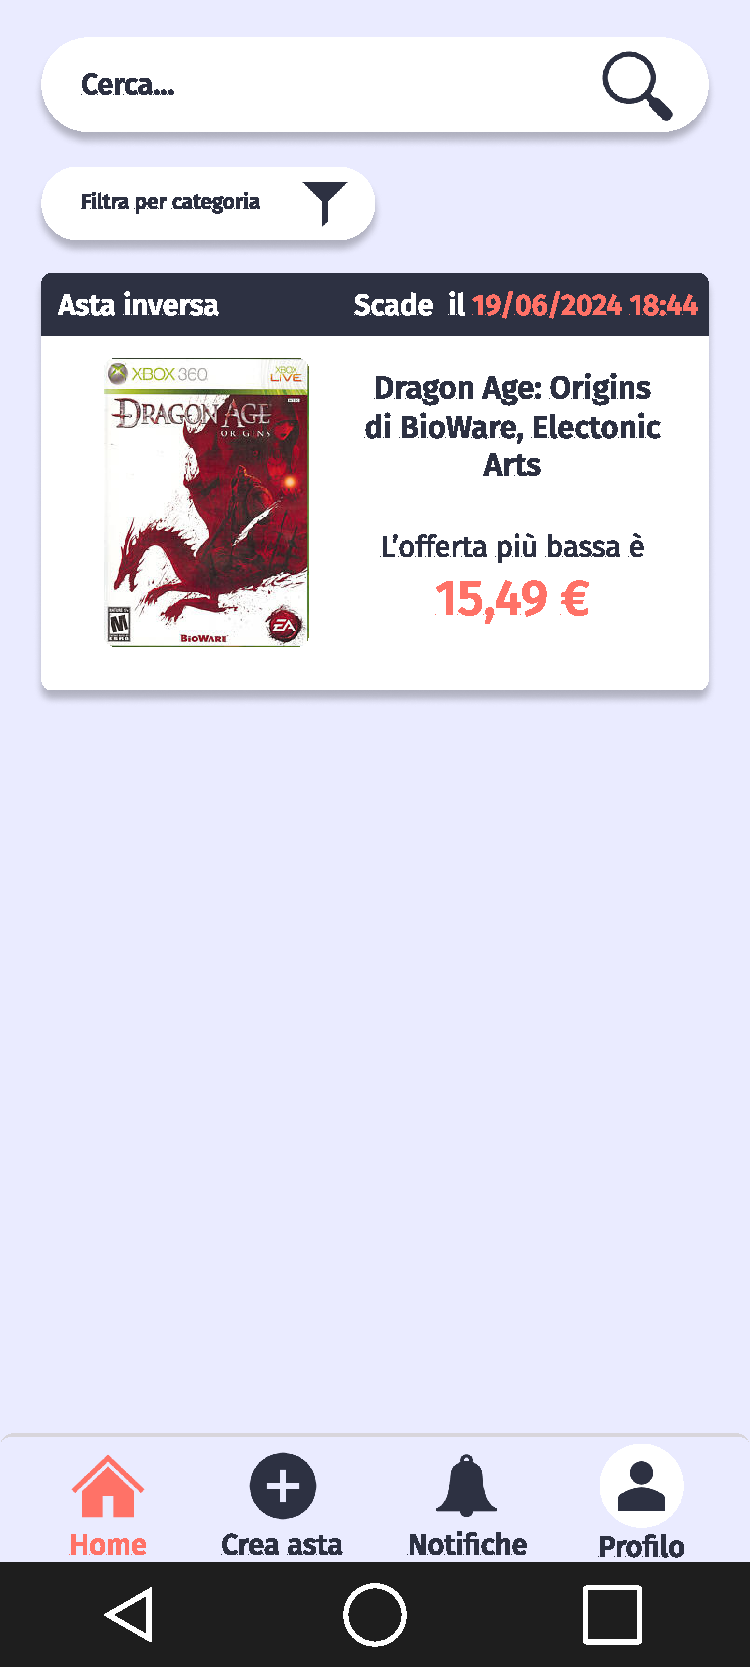
\includegraphics[width=.7\linewidth]{Immagini/Frames/Venditore/V1.pdf}
                    \caption{Home venditore}
            \end{minipage}\hfill
            \begin{minipage}{0.32\textwidth}
                \centering
                \includegraphics[width=.7\linewidth]{Immagini/Frames/Venditore/V7.pdf}
                \caption{Menu profilo venditore}
            \end{minipage}\hfill
            \begin{minipage}{0.32\textwidth}
                \centering
                \includegraphics[width=.7\linewidth]{Immagini/Frames/Venditore/V11.pdf}
                \caption{Aste create venditore}
            \end{minipage}\hfill
        \end{figure}
    
        \begin{figure}[!htb]
            \begin{minipage}{0.32\textwidth}
                \centering
                \includegraphics[width=.7\linewidth]{Immagini/Frames/Venditore/V13.pdf}
                \caption{Offerte ricevute asta silenziosa}
            \end{minipage}\hfill
            \begin{minipage}{0.32\textwidth}
                \centering
                \includegraphics[width=.7\linewidth]{Immagini/Frames/Popup/P7.pdf}
                \caption{Conferma accettazione offerta}
            \end{minipage}\hfill
            \begin{minipage}{0.32\textwidth}
                \centering
                \includegraphics[width=.7\linewidth]{Immagini/Frames/Venditore/V14.pdf}
                \caption{Offerte ricevute asta silenziosa dopo aver accettato un'offerta}
            \end{minipage}\hfill
        \end{figure}
    
        \begin{figure}[!htb]
            \begin{minipage}{0.32\textwidth}
                \centering
                \includegraphics[width=.7\linewidth]{Immagini/Frames/Venditore/V17.pdf}
                \caption{Dettagli asta selezionata}
            \end{minipage}\hfill
            \begin{minipage}{0.32\textwidth}
                \centering
                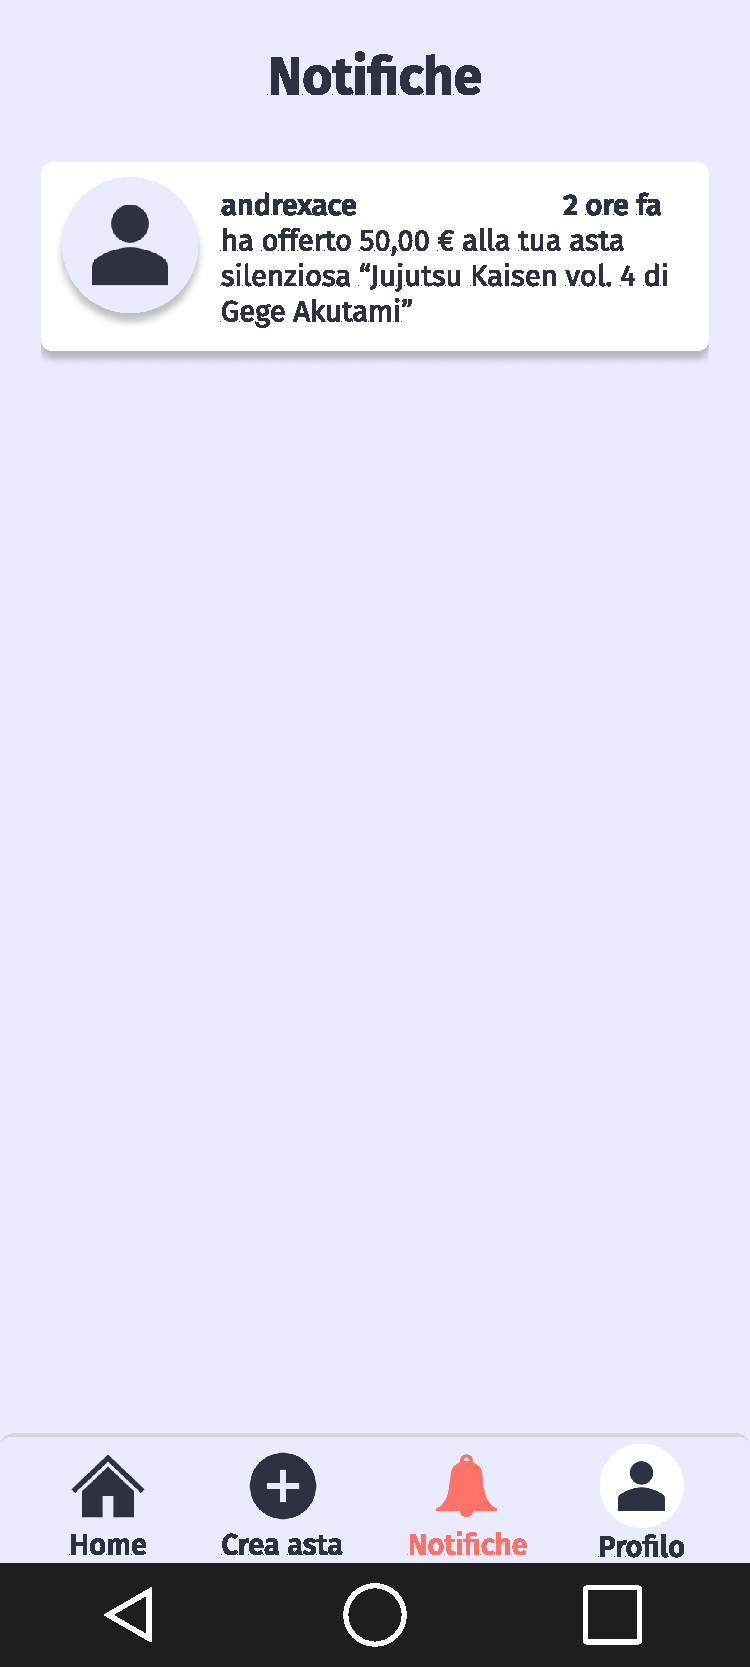
\includegraphics[width=.7\linewidth]{Immagini/Frames/Venditore/V6.pdf}
                \caption{Notifiche}
            \end{minipage}\hfill
        \end{figure}

    \clearpage
    
    \section{Valutazione dell’usabilità a priori}
        La valutazione dell'usabilità consiste nel verificare l'aderenza dell'interfaccia alle 8 regole d'oro di Ben Shneiderman o alle 10 euristiche di Nielsen. In particolare, alcuni punti forti individuati sono stati:
        \begin{itemize}
            \item Consistenza: Lo stile dell'applicazione, sia nei colori che nelle dimensioni di font ed elementi dell'interfaccia rimane costante e coerente.
            \item Standard: L'interfaccia utilizza convenzioni dell'industria sia nel posizionamento degli elementi sull'interfaccia e sia nelle icone utilizzate.
            \item Scorciatoie: L'applicazione permette agli utenti di effettuare delle operazioni con un numero estremamente basso di tap e re-direzioni.
            \item Messaggi informativi: L'applicazione permette agli utenti di essere a conoscenza di esiti negativi delle loro operazioni grazie a dei pop-up informativi. Lo stesso vale per l'esito positivo di una operazione.
            \item Memoria a breve termine: L'applicazione ha un'interfaccia minimale senza troppi ingombri visivi che possono sovraccaricare la memoria a breve termine dell'utente; in tal modo non si sentirà disorientato dalla mole di informazioni mostrate su schermo.
            \item Corrispondenza con il mondo reale: L'applicazione utilizza un linguaggio semplice e non costringe gli utenti ad informarsi attraverso fonti esterne per comprendere ciò che gli viene mostrato.
            \item Controllo dell'utente e prevenzione errori: L'applicazione impedisce all'utente di effettuare delle operazioni importanti senza prima richiedere una conferma, così da consentire di cambiare idea oppure prevenire errori di tap.
            \item Aiuto e documentazione: L'applicazione fornisce una sezione di aiuto interna che permette all'utente di capire come effettuare passo per passo ogni operazione più importante.
        \end{itemize}
    
        \subsection{Valutazioni con utenti}
            Sono stati effettuati una serie di valutazioni di usabilità attraverso i prototipi costruiti con Figma. \\
            In particolare, nelle tabelle seguenti sono riportati i casi d'uso testati e, per ogni utente, viene indicato con:
            \begin{itemize}
                \item S = Successo (ovvero la task è stata completata velocemente e senza intoppi)
                \item P = Successo parziale (ovvero è stato necessario un po' di tempo in più e piccoli suggerimenti)
                \item F = Fallimento (ovvero la task non è stata completata nonostante i piccoli suggerimenti)
                \item X = Non testato
            \end{itemize}
        
            \begin{table}[ht]
            \resizebox{\textwidth}{!}{
                \begin{tabular}{l|l|l|l|l|l|l|l|l|l|}
                \cline{2-10}
                &
                \begin{tabular}[c]{@{}l@{}}Registrazione\\ account\end{tabular} &
                \begin{tabular}[c]{@{}l@{}}Accesso\\ account\end{tabular} &
                \begin{tabular}[c]{@{}l@{}}Ricerca\\ aste\end{tabular} &
                \begin{tabular}[c]{@{}l@{}}Filtra\\ aste\end{tabular} &
                \begin{tabular}[c]{@{}l@{}}Visualizza\\ dettagli asta\end{tabular} &
                \begin{tabular}[c]{@{}l@{}}Visualizza\\ profilo\\ proprietario\\ asta\end{tabular} &
                \begin{tabular}[c]{@{}l@{}}Visualizza\\ le tue aste\\ create\end{tabular} &
                \begin{tabular}[c]{@{}l@{}}Modifica\\ la tua\\ asta\end{tabular} &
                \begin{tabular}[c]{@{}l@{}}Elimina\\ la tua\\ asta\end{tabular}\\ \hline
                \multicolumn{1}{|l|}{Utente 1} & S & S & S & S & S & S & S & S & S \\ \hline
                \multicolumn{1}{|l|}{Utente 2} & S & S & S & P & S & P & S & S & S \\ \hline
                \multicolumn{1}{|l|}{Utente 3} & S & S & S & S & S & S & S & S & S \\ \hline
                \multicolumn{1}{|l|}{Utente 4} & S & S & S & S & S & P & S & S & S \\ \hline
                \multicolumn{1}{|l|}{Utente 5} & S & S & S & S & P & P & P & S & S \\ \hline
                \multicolumn{1}{|l|}{Utente 6} & S & S & S & S & P & S & P & S & S \\ \hline %Kevin
                \multicolumn{1}{|l|}{Utente 7} & S & S & X & X & P & P & S & S & S \\ \hline %Nancy
                \multicolumn{1}{|l|}{Utente 8} & S & S & S & S & S & S & P & S & S \\ \hline %Cristina
                \multicolumn{1}{|l|}{Utente 9} & S & S & X & X & S & S & S & P & S \\ \hline %Francesco
                \end{tabular}
                }
            \end{table}
            
            \begin{table}[ht]
            \resizebox{\textwidth}{!}{
                \begin{tabular}{l|l|l|l|l|l|l|l|l|}
                \cline{2-9}
                &
                \begin{tabular}[c]{@{}l@{}}Visualizza\\ il tuo\\ profilo\end{tabular} &
                \begin{tabular}[c]{@{}l@{}}Visualizza\\ aste a cui\\ hai\\ partecipato\end{tabular} &
                \begin{tabular}[c]{@{}l@{}}Modifica\\ il tuo\\ profilo\end{tabular} &
                \begin{tabular}[c]{@{}l@{}}Visualizza\\ offerte per\\ la tua asta\end{tabular} &
                \begin{tabular}[c]{@{}l@{}}Fai un'offerta\\ ad un'asta\end{tabular} &
                \begin{tabular}[c]{@{}l@{}}Crea\\ asta\end{tabular} &
                \begin{tabular}[c]{@{}l@{}}Accetta\\ offerte\\ asta\\ silenziosa\end{tabular} &
                \begin{tabular}[c]{@{}l@{}}Rifiuta\\ offerte\\ asta\\ silenziosa\end{tabular}\\ \hline
                \multicolumn{1}{|l|}{Utente 1} & S & S & S & S & S & S & X & X \\ \hline
                \multicolumn{1}{|l|}{Utente 2} & S & S & P & S & S & S & X & X \\ \hline
                \multicolumn{1}{|l|}{Utente 3} & S & S & P & S & S & S & S & S \\ \hline
                \multicolumn{1}{|l|}{Utente 4} & S & S & P & S & S & S & S & S \\ \hline
                \multicolumn{1}{|l|}{Utente 5} & S & F & P & S & S & S & S & S \\ \hline
                \multicolumn{1}{|l|}{Utente 6} & S & P & F & S & X & S & X & X \\ \hline %Kevin
                \multicolumn{1}{|l|}{Utente 7} & P & S & P & S & X & S & X & X \\ \hline %Nancy
                \multicolumn{1}{|l|}{Utente 8} & S & P & S & S & S & S & X & X \\ \hline %Cristina
                \multicolumn{1}{|l|}{Utente 9} & S & S & S & S & S & S & X & X \\ \hline %Francesco
                \end{tabular}
                }
            \end{table}
            
            Al fine di quantificare la bontà di realizzazione dell'interfaccia e la riposta degli utenti ad essa (in particolare il primo, utilizzeremo un sistema di punteggio per ogni caso d'uso. \\
            Il punteggio è riferito al primo test di usabilità sulla prima versione del prototipo. \\
            Il campione di utenti in esame distingue ogni individuo per sesso, età, livello di inclinazione al digitale e contesto familiare.
            
            \noindent In particolare seguiremo le seguenti regole:
            \begin{itemize}
                \item Per ogni caso d'uso, il punteggio massimo attribuibile è da 0 ad N (dove N è il numero di utenti che hanno testato quel caso d'uso).
                \item Se l'utente ha testato il caso d'uso con successo (S), si somma al totale 1.
                \item Se l'utente ha testato il caso d'uso con parziale successo (P), si somma al totale 0,5.
                \item Se l'utente ha testato il caso d'uso con insuccesso (F), si somma al totale 0.
                \item Si calcola infine per ogni caso d'uso la percentuale di successo così:
                \vspace{0.5cm} \\
                $\displaystyle\frac{\sum_{utente = 1} ^{N}punteggio(utente)}{\sum_{utente = 1} ^{N}1} = \frac{punteggioOttenuto}{punteggioTotale}$.
            \end{itemize}

            \vspace{0.5cm}
            
            \noindent Le percentuali di successo per ogni caso d'uso testato al sono:
            \begin{itemize}
                \item Registrazione account: $\frac{9}{9} = 1 = 100\%$
                \item Accesso account: $\frac{9}{9} = 1 = 100\%$
                \item Ricerca aste: $\frac{7}{7} = 1 = 100\%$
                \item Filtra aste: $\frac{6,5}{7} = 0,93 = 93\%$
                \item Visualizza dettagli asta: $\frac{7,5}{9} = 0,83 = 83\%$
                \item Visualizza profilo proprietario asta: $\frac{7}{9} = 0,78 = 78\%$
                \item Visualizza le tue aste create: $\frac{7,5}{9} = 0,83 = 83\%$
                \item Modifica la tua asta: $\frac{8,5}{9} = 0,94 = 94\%$
                \item Elimina la tua asta: $\frac{9}{9} = 1 = 100\%$
                \item Visualizza il tuo profilo: $\frac{8,5}{9} = 0,94 = 94\%$
                \item Visualizza asta a cui hai partecipato: $\frac{7}{9} = 0,78 = 78\%$
                \item Modifica il tuo profilo: $\frac{6,5}{9} = 0,72 = 72\%$
                \item Visualizza offerte per la tua asta: $\frac{9}{9} = 1 = 100\%$
                \item Fai un'offerta ad un'asta: $\frac{7}{7} = 1 = 100\%$
                \item Crea asta: $\frac{9}{9} = 1 = 100\%$
                \item Accetta offerte asta silenziosa: $\frac{3}{3} = 1 = 100\%$
                \item Rifiuta offerte asta silenziosa: $\frac{3}{3} = 1 = 100\%$
            \end{itemize}
        
        \subsection{Modifiche a seguito delle valutazioni}
            Dalle valutazioni effettuate, sono state riscontrate alcune criticità che hanno comportato una rielaborazione di alcuni aspetti dell’interfaccia. \\
            Dopo la risoluzione di tali problemi, il tasso di successo ha registrato un incremento.

            \begin{center}
            \begin{longtable}{|C{7.35cm}|C{7.35cm}|}
                \hline
                    \textbf{Problematica riscontrata} & \textbf{Modifica apportata}\\
                \hline
                \endhead
                    La presenza dello sfondo bianco sotto le singole informazioni delle "informazioni utente" ha indotto alcuni soggetti a cliccare direttamente i campi per effettuare una modifica, ignorando la presenza del pulsantino apposito. &
                    Abbiamo rimosso lo sfondo bianco da tutti gli elementi non cliccabili, concentrando l’attenzione del soggetto solo ed esclusivamente sul pulsante di modifica apposito. \\
                \hline
                    All'interno della schermata "home", la presenza di un nome utente all’interno della scheda di anteprima subito al di sotto dell’offerta più elevata ha erroneamente indotto alcuni soggetti a pensare che quell’utente fosse l’offerente del prezzo, e non il creatore dell’asta come inteso. &
                    Abbiamo rimosso il nome dell’utente nelle schede di anteprima delle aste specificandolo solo ed esclusivamente nei dettagli dell’asta, preceduto dalla dicitura “Creata da”. \\
                \hline
                    La presenza della propria asta creata all’interno della "home" ha confuso un soggetto e lo ha spinto a voler offrire una somma di denaro per suddetta asta, quando invece ciò non è possibile essendone lui stesso il creatore. &
                    Abbiamo rimosso dalla "home" le aste a cui l’utente non può partecipare, ossia le aste create da altri account dello stesso tipo e le aste da lui stesso create. \\
                \hline
                    La presenza del tasto "home" nella barra di navigazione dell’applicazione ha portato alcuni soggetti a cliccare su di essa per tornare alla schermata principale una volta effettuata una ricerca per parola chiave o per categoria, ignorando il tasto indietro apposito (del dispositivo). &
                    Abbiamo reso il pulsante "home" utilizzabile anche per tornare alla schermata principale una volta effettuata una ricerca per parola chiave o per categoria.\\
                \hline
                    La presenza di inglesismi (logout, guest) ha confuso i soggetti più anziani, ignari del significato della parola. &
                    Abbiamo reso la nostra applicazione completamente in italiano.\\
                \hline
                    Un utente ha provato ad effettuare lo zoom sulle immagini con un pinch out anziché toccando l’immagine stessa. & 
                    Tale azione sarà implementata nell'applicazione finale.\\
                \hline
                    Nella sezione "Aiuto", alcuni utenti hanno cliccato sulla parte bianca del pulsante per accedere ai singoli pop-up informativi; quando era inteso cliccare solo sulla freccia blu. &
                    Abbiamo reso cliccabili ogni singolo pulsante bianco nella sezione "Aiuto".\\
                \hline
                    Un utente non esperto del dominio desiderava conoscere quali fossero le caratteristiche di un determinato tipo di asta direttamente dai dettagli dell'asta e non andando a cercare nella sezione "Aiuto". &
                    Abbiamo aggiunto un "?" che rimanda alle informazioni sul tipo di asta visualizzata. Tale bottone si trova vicino al tipo di asta nella sezione "Dettagli asta", raggiungibile cliccando sul'anteprima di un'asta nella "Home".\\
                \hline
                    Un utente ha trovato difficoltà nel modificare il profilo poichè non vedeva il bottone dedicato a tale funzionalità. In particolare, ha cercato il bottone nella parte bassa dello schermo. &
                    Abbiamo spostato il bottone di "modifica profilo" rendendolo un bottone in sovrimpressione in basso a destra all'interno della sezione delle "informazioni utente". \\
                \hline
            \end{longtable}
            \end{center}
    %PDF DI RIFERIMENTO: 04_Modelli di Dominio.pdf, Statecharts.pdf

\chapter{Requirement Specification}
    \section{Obiettivo}
        I requisiti che sono stati riorganizzati nella fase di analisi sono formalizzati in diagrammi (diagramma di classe, diagramma di sequenza, diagramma degli stati) attraverso l'uso di linguaggi di modellazione come UML. \\
        Per individuare il modello ad oggetti per questo dominio, si è scelto di impiegare l'euristica "Three-Object-Type" perché permette di costruire un modello più flessibile e facile da modificare.

    \section{Class Diagram}
        Il Class Diagram individua quali sono le entità coinvolte all'interno del nostro dominio e le relazioni che tra esse sussistono.\\
        In particolare, il modello concettuale basato sull'analisi dei requisiti permetterà di creare un modello efficace per la gestione delle aste.\\
        \subsection{Class Diagram del dominio del problema}
            %Class Diagram costruito con StarUML
            \begin{figure}[htbp!]
                \centering
                    \includegraphics[width=1\linewidth]{Immagini/Diagrammi/Class Diagram/ClassDiagramDominio.pdf}
                \caption{Class Diagram del dominio del problema}
                \label{fig:Class Diagram del dominio del problema}
            \end{figure}
            
        \subsection{Class Diagram per casi d'uso}
            In questa sezione verranno mostrati i diagrammi secondo l'euristica "Three-Object-Type" per ogni caso d'uso. Le classi possono essere di tipo "boundary", "control" e "entity".
        
            \begin{figure}[htbp!]
                \centering
                    \includegraphics[width=1\linewidth]{Immagini/Diagrammi/Class Diagram/Utente che non ha effettuato l'accesso/ScelteIniziali.pdf}
                \caption{Scelta del tipo di account}
            \end{figure}
            
            \begin{figure}[htbp!]
                \centering
                    \includegraphics[width=0.35\linewidth]{Immagini/Diagrammi/Class Diagram/Utente che non ha effettuato l'accesso/Accesso.pdf}
                \caption{Accesso}
            \end{figure}
            
            \begin{figure}[htbp!]
                \centering
                    \includegraphics[width=0.55\linewidth]{Immagini/Diagrammi/Class Diagram/Utente che non ha effettuato l'accesso/Registrazione.pdf}
                \caption{Registrazione}
            \end{figure}
            
            \begin{figure}[htbp!]
                \centering
                    \includegraphics[width=1\linewidth]{Immagini/Diagrammi/Class Diagram/Utente che non ha effettuato l'accesso/CreazioneProfilo.pdf}
                \caption{Creazione del profilo}
            \end{figure}
            
            \begin{figure}[htbp!]
                \centering
                    \includegraphics[width=1\linewidth]{Immagini/Diagrammi/Class Diagram/Utente generico/RicercaCategoria.pdf}
                \caption{Ricerca per categoria}
            \end{figure}
            
            \begin{figure}[htbp!]
                \centering
                    \includegraphics[width=1\linewidth]{Immagini/Diagrammi/Class Diagram/Utente generico/RicercaParolaChiave.pdf}
                \caption{Ricerca per parola chiave}
            \end{figure}
            
            \begin{figure}[htbp!]
                \centering
                    \includegraphics[width=1\linewidth]{Immagini/Diagrammi/Class Diagram/Utente generico/RicercaParolaChiaveCategoria.pdf}
                \caption{Ricerca per parola chiave e categoria}
            \end{figure}
            
            \begin{figure}[htbp!]
                \centering
                    \includegraphics[width=1\linewidth]{Immagini/Diagrammi/Class Diagram/Utente generico/VisualizzaAsteAttive.pdf}
                \caption{Visualizza aste attive}
            \end{figure}
            
            \begin{figure}[htbp!]
                \centering
                    \includegraphics[width=1\linewidth]{Immagini/Diagrammi/Class Diagram/Utente generico/VisualizzaDettagliAstaUtente.pdf}
                \caption{Visualizza dettagli asta di un altro utente}
            \end{figure}
            
            \begin{figure}[htbp!]
                \centering
                    \includegraphics[width=1\linewidth]{Immagini/Diagrammi/Class Diagram/Utente generico/VisualizzaProfiloUtente.pdf}
                \caption{Visualizza profilo utente}
            \end{figure}
            
            \begin{figure}[htbp!]
                \centering
                    \includegraphics[width=1\linewidth]{Immagini/Diagrammi/Class Diagram/Utente che ha effettuato l'accesso/EliminaAsta.pdf}
                \caption{Elimina asta creata}
            \end{figure}
            
            \begin{figure}[htbp!]
                \centering
                    \includegraphics[width=1\linewidth]{Immagini/Diagrammi/Class Diagram/Utente che ha effettuato l'accesso/ModificaAstaTempoFisso.pdf}
                \caption{Modifica asta a tempo fisso}
            \end{figure}
            
            \begin{figure}[htbp!]
                \centering
                    \includegraphics[width=1\linewidth]{Immagini/Diagrammi/Class Diagram/Utente che ha effettuato l'accesso/ModificaAstaInversa.pdf}
                \caption{Modifica asta inversa}
            \end{figure}
            
            \begin{figure}[htbp!]
                \centering
                    \includegraphics[width=1\linewidth]{Immagini/Diagrammi/Class Diagram/Utente che ha effettuato l'accesso/ModificaAstaSilenziosa.pdf}
                \caption{Modifica asta silenziosa}
            \end{figure}
            
            \begin{figure}[htbp!]
                \centering
                    \includegraphics[width=0.8\linewidth]{Immagini/Diagrammi/Class Diagram/Utente che ha effettuato l'accesso/ModificaProfilo.pdf}
                \caption{Modifica profilo}
            \end{figure}

            \begin{figure}[htbp!]
                \centering
                    \includegraphics[width=0.5\linewidth]{Immagini/Diagrammi/Class Diagram/Utente che ha effettuato l'accesso/SceltaCreazioneAsta.pdf}
                \caption{Scelta tipo di asta da creare}
            \end{figure}
            
            \begin{figure}[htbp!]
                \centering
                    \includegraphics[width=1\linewidth]{Immagini/Diagrammi/Class Diagram/Utente che ha effettuato l'accesso/VisualizzaAsteCreate.pdf}
                \caption{Visualizza aste create}
            \end{figure}

            \begin{figure}[htbp!]
                \centering
                    \includegraphics[width=1\linewidth]{Immagini/Diagrammi/Class Diagram/Utente che ha effettuato l'accesso/VisualizzaDettagliPropriaAsta.pdf}
                \caption{Visualizza dettagli della propria asta}
            \end{figure}
            
            \begin{figure}[htbp!]
                \centering
                    \includegraphics[width=1\linewidth]{Immagini/Diagrammi/Class Diagram/Utente che ha effettuato l'accesso/VisualizzaMenuProfilo.pdf}
                \caption{Visualizza menu profilo}
            \end{figure}
            
            \begin{figure}[htbp!]
                \centering
                    \includegraphics[width=1\linewidth]{Immagini/Diagrammi/Class Diagram/Utente che ha effettuato l'accesso/VisualizzaNotifiche.pdf}
                \caption{Visualizza notifiche}
            \end{figure}
            
            \begin{figure}[htbp!]
                \centering
                    \includegraphics[width=1\linewidth]{Immagini/Diagrammi/Class Diagram/Utente che ha effettuato l'accesso/VisualizzaOfferteRicevute.pdf}
                \caption{Visualizza offerte ricevute}
            \end{figure}
            
            \begin{figure}[htbp!]
                \centering
                    \includegraphics[width=0.75\linewidth]{Immagini/Diagrammi/Class Diagram/Utente che ha effettuato l'accesso/VisualizzaProprioProfilo.pdf}
                \caption{Visualizza profilo personale}
            \end{figure}
            
            \begin{figure}[htbp!]
                \centering
                    \includegraphics[width=1\linewidth]{Immagini/Diagrammi/Class Diagram/Utente che ha effettuato l'accesso/VisualizzaStoricoPartecipazioni.pdf}
                \caption{Visualizza aste partecipate}
            \end{figure}
            
            \begin{figure}[htbp!]
                \centering
                    \includegraphics[width=1\linewidth]{Immagini/Diagrammi/Class Diagram/Venditore e compratore/AccettaRifiutaOffertaSilenziosa.pdf}
                \caption{Accetta o rifiuta un'offerta per un'asta silenziosa}
            \end{figure}
            
            \begin{figure}[htbp!]
                \centering
                    \includegraphics[width=1\linewidth]{Immagini/Diagrammi/Class Diagram/Venditore e compratore/CreaAstaFissa.pdf}
                \caption{Crea un'asta a tempo fisso}
            \end{figure}
            
            \begin{figure}[htbp!]
                \centering
                    \includegraphics[width=1\linewidth]{Immagini/Diagrammi/Class Diagram/Venditore e compratore/CreaAstaInversa.pdf}
                \caption{Crea un'asta inversa}
            \end{figure}
            
            \begin{figure}[htbp!]
                \centering
                    \includegraphics[width=1\linewidth]{Immagini/Diagrammi/Class Diagram/Venditore e compratore/CreaAstaSilenziosa.pdf}
                \caption{Crea un'asta silenziosa}
            \end{figure}
            
            \begin{figure}[htbp!]
                \centering
                    \includegraphics[width=1\linewidth]{Immagini/Diagrammi/Class Diagram/Venditore e compratore/FaiOfferta.pdf}
                \caption{Fai un'offerta}
            \end{figure}

    \clearpage
        
    \section{Dizionario delle classi}
        \begin{tabular}{|C{3.5cm}|L{11.2cm}|}
            \hline
            \multicolumn{1}{|c|}{\textbf{Classe}} & \multicolumn{1}{c|}{\textbf{Descrizione}}\\  
            \hline
                Account &
                Cosa rappresenta la classe\\
            \hline
                Venditore &
                Cosa rappresenta la classe\\
            \hline
                Compratore &
                Cosa rappresenta la classe\\
            \hline
                Profilo &
                Cosa rappresenta la classe\\
            \hline
                Notifica &
                Cosa rappresenta la classe\\
            \hline
                Asta &
                Cosa rappresenta la classe\\
            \hline
                Asta di compratore &
                Cosa rappresenta la classe\\
            \hline
                Asta di venditore &
                Cosa rappresenta la classe\\
            \hline
                Asta a tempo fisso &
                Cosa rappresenta la classe\\
            \hline
                Asta silenziosa &
                Cosa rappresenta la classe\\
            \hline
                Asta inversa &
                Cosa rappresenta la classe\\
            \hline
                Offerta &
                Cosa rappresenta la classe\\
            \hline
                Offerta di compratore &
                Cosa rappresenta la classe\\
            \hline
                Offerta di venditore &
                Cosa rappresenta la classe\\
            \hline
                Offerta a tempo fisso &
                Cosa rappresenta la classe\\
            \hline
                Offerta silenziosa &
                Cosa rappresenta la classe\\
            \hline
                Offerta inversa &
                Cosa rappresenta la classe\\
            \hline
        \end{tabular}
        
    \section{Dizionario delle associazioni}
        \begin{tabular}{|C{3.5cm}|L{11.2cm}|}
            \hline
                \multicolumn{1}{|c|}{\textbf{Associazione}} &
                \multicolumn{1}{c|}{\textbf{Descrizione}}\\            
            \hline
                Mittente &
                Cosa rappresenta l'associazione\\
            \hline
                Destinatario &
                Cosa rappresenta l'associazione\\
            \hline
                Possiede &
                Cosa rappresenta l'associazione\\
            \hline
                È associata a &
                Cosa rappresenta l'associazione\\
            \hline
                Possiede &
                Cosa rappresenta l'associazione\\
            \hline
                È collegato a &
                Cosa rappresenta l'associazione\\
            \hline
                Possiede &
                Cosa rappresenta l'associazione\\
            \hline
                È collegato a &
                Cosa rappresenta l'associazione\\
            \hline
                Si riferisce a &
                Cosa rappresenta l'associazione\\
            \hline
                Si riferisce a &
                Cosa rappresenta l'associazione\\
            \hline
                Si riferisce a &
                Cosa rappresenta l'associazione\\
            \hline
        \end{tabular}

    \section{Sequence Diagram}
        Il diagramma di sequenza rappresenta i processi e gli oggetti coinvolti e la sequenza dei messaggi scambiati necessari per adempiere ad una funzionalità. \\
        Le interazioni sono disposte lungo un'asse temporale per dare un'idea dell'ordine di avvicendamento dei messaggi.
        
        \begin{figure}[htbp!]
        \centering
            \includegraphics[width=1\linewidth]{Immagini/Diagrammi/Sequence Diagram/CreaAstaInversa.pdf}
        \caption{Sequence Diagram creazione asta inversa}
        \end{figure}

        \begin{figure}[htbp!]
        \centering
            \includegraphics[width=1\linewidth]{Immagini/Diagrammi/Sequence Diagram/AccettaOffertaSilenziosa.pdf}
        \caption{Sequence Diagram accetta offerta per un'asta silenziosa}
        \end{figure}

    \clearpage
    
    \section{Statechart Diagram}
        Il diagramma degli stati consente di rappresentare gli aspetti dinamici di un sistema, in particolare per l'interfaccia utente. \\
        Presenta quindi una serie di stati che il sistema attraversa (come una macchina a stati finiti), le azioni che comportano una transizione da uno stato all'altro, e le condizioni da rispettare affinché la transizione possa avvenire.

            \begin{figure}[htbp!]
            \centering
                \includegraphics[width=0.1\linewidth]{Immagini/WorkInProgress.pdf}
            \caption{Statechart Diagram creazione asta inversa}
            \end{figure}
            
            \begin{figure}[htbp!]
            \centering
                \includegraphics[width=0.1\linewidth]{Immagini/WorkInProgress.pdf}
            \caption{Statechart Diagram accetta offerta per un'asta silenziosa}
            \end{figure}
    \chapter{Usabilità}
    \section{Usabilità}

    \section{Test di usabilità} %Test di usabilità con varie persone

    \section{Miglioramenti a seguito dei test di usabilità}
    %PDF DI RIFERIMENTO: 06_System Design.pdf + DesignPractices.pdf, 08_Architetture Software.pdf, 08_Architetture.pdf, XX-REST-APIs.pdf

\chapter{System Design}
    \section{Architettura utilizzata}
        Architettura a tre livelli

    \section{Elenco REST API utilizzate}
    %PDF DI RIFERIMENTO: 06_System Design.pdf + DesignPractices.pdf, 08_Architetture Software.pdf, 08_Architetture.pdf

\chapter{Object Design}
    La progettazione orientata agli oggetti è la fase di sviluppo del software nella quale si definisce il dettaglio implementativo dei vari sottosistemi. \\
    Tali sottosistemi devono soddisfare i requisiti non funzionali di performance, affidabilità e manutenibilità. Sono costruiti sulla base degli oggetti individuati nel dominio del problema, ai quali inevitabilmente saranno aggiunti nuovi oggetti per giungere alla soluzione. \\
    Le scelte adoperate hanno l'obiettivo di favorire il basso accoppiamento tra i sottosistemi e la manutenibilità, in modo da mantenere un'alta qualità interna del software.

    \section{Design Pattern}
        \subsection{Client}
            Il client possiede un'architettura con due strati: lo \textbf{strato della UI} e lo \textbf{strato dei dati}. \\
            Nel complesso, è un ibrido tra il pattern \textbf{MVVM} (Model-View-ViewModel) e \textbf{MVC} (Model-View-Controller).

            \begin{figure}[htbp!]
                \centering
                \includegraphics[width=0.45\linewidth]{Immagini/Object Design/ArchitetturaClient.pdf}
                \caption{Schema dell'architettura adottata (client)}
            \end{figure}
            
            \begin{itemize}
                \item Lo strato della UI comprende \textbf{View}, \textbf{StateHolder} (che mantengono i dati sullo stato della View, come i \textbf{ViewModel}) e \textbf{Controller} e si occupa di gestire l'interfaccia e l'interazione con l'utente.
                    \begin{itemize}
                        \item Le \textit{View} sono dei file .XML che utilizzano degli schemi definiti da Android per la creazione dell'interfaccia utente. Inoltre, grazie al View binding, per ogni vista viene generata una classe Java che contiene riferimenti a tutti gli elementi della vista per poter interagire con essa. Esse interagiscono con il Controller per chiamare i metodi che gestiscono l'interazione con l'utente.
                        \item I \textit{ViewModel} sono delle classi che hanno il compito di mantenere i dati che devono essere mostrati sulla UI. L'utilizzo del ViewModel è essenziale per poter mantenere i dati anche in caso di cambiamenti dello stato dell'applicazione, come rotazioni dello schermo o riduzione ad attività in secondo piano. I ViewModel, che nella architettura MVVM interagiscono direttamente con il Model e si interpongono tra quest'ultimo e la View, eseguono anche operazioni sui dati, come il recupero dei dati paginati da mostrare sullo schermo e la validazione dei dati inseriti dall'utente.
                        \item L'aggiunta del \textit{Controller} è ciò che rende ibrida questa architettura. Il Controller si interpone tra ViewModel e View per separare i compiti che riguardano il conservare e il convalidare i dati della vista (affidati al ViewModel) da altre operazioni, come appunto le risposte all'interazione con l'utente, la creazione di messaggi di errore, e l'invio di richieste non relative a dati da mostrare, come ad esempio l'autenticazione. Inoltre esso funge da osservatore ai dati che sono presenti nel ViewModel e, in caso di mutazione, provvede ad aggiornare la vista con tali nuovi dati.
                    \end{itemize}
                \item Lo strato dei dati è rappresentato dal \textbf{Model} e il suo ruolo è comunicare con le fonti di dati, siano esse esterne (come basi di dati) che locali (come cache o basi di dati interne). Il Model, a sua volta, è organizzato secondo il pattern \textbf{Repository}, con tre sottostrati: \textbf{Repository}, \textbf{Service} e \textbf{ServiceImpl}.
                    \begin{itemize}
                        \item Le classi \textit{Repository} rappresentano una enumerazione delle operazioni che la logica dell'applicazione può effettuare sui dati, chiamando poi attraverso le interfacce Service i metodi che svolgono l'effettivo lavoro sui dati.
                        \item Le classi \textit{Service} rappresentano una interfaccia che astrae queste operazioni sui dati. In questo caso, esse rappresentano una interfaccia di metodi che verranno utilizzati per la creazione di richieste HTTP da inviare agli endpoint del backend.
                        \item Le classi \textit{ServiceImpl} rappresentano dei metodi concreti - implementati dalla libreria Retrofit - che, sulla base delle annotazioni e i parametri inseriti nelle interfacce dei metodi di Service, creeranno la giusta richiesta HTTP da inviare al backend.
                    \end{itemize}
            \end{itemize}
    
        \subsection{Resource Server}
            L'architettura adottata per il sottosistema \textbf{Resource Server} (da qui in avanti chiamato semplicemente \textbf{Server}) è un'architettura di tipo \textbf{esagonale}. L'obiettivo di tale architettura è di definire una \textbf{separazione netta} tra la business logic del dominio (anche detto \textit{domain layer}) e tutto ciò che sono i fattori esterni, ovvero il layer di interfaccia con l'utente (anche detto \textit{application layer}) e il layer di persistenza (anche detto \textit{infrastracture layer}), attraverso una serie di interfacce ben definite. \\
            L'obiettivo di tale scelta è quello di migliorare la manutenibilità, la scalabilità e la modularità del backend, definendo così interfacce ben definite che permettono a più team di sviluppo di lavorare parallelamente, conoscendo esattamente il contratto per le interazioni tra la logica del dominio e dei protocolli di comunicazione tra l'applicazione e i suoi adattatori. \cite{AppMaster1}
            
            In particolare, il design pattern adottato per il domain layer è di tipo \textbf{Domain Driven}. Un approccio di tipo Domain Driven permette di avere un'\textbf{alta coesione} e \textbf{ridurre al minimo l'accoppiamento} tra le classi della business logic, dando a ciascuna classe del domain layer un solo motivo per cambiare: un cambiamento nell'entità del dominio corrispondente.
            \begin{figure}[htbp!]
                \centering
                \includegraphics[width=0.8\linewidth]{Immagini/Object Design/DDD-Layers.jpg}
                \caption{Schema dell'architettura adottata (backend)}
                \cite{Baeldung1}
            \end{figure}

            In particolare, il backend è così organizzato:
            \begin{itemize}
                \item L'\textit{application layer} contiene le classi responsabili di esporre le REST API che verranno chiamate dall'utente. E' dipendente solo e unicamente da classi DTO, che si occupano di raccogliere le informazioni ricevute sottoforma di HTTP Request e saranno tradotte in HTTP Response. \cite{Baeldung2}
                \item Il \textit{domain layer} contiene le classi responsabili della business logic, che dipende solo e unicamente dalle classi del dominio, ovvero le entità. Al suo interno troviamo anche classi responsabili di tradurre i DTO in entità del dominio. \\
                Inoltre, grazie all'interfaccia offerta dalla \textbf{Java Persistance API}, le classi necessarie per la comunicazione con il persistance layer sono gestite da Spring Boot attraverso una Spring dependency.
                \item Il \textit{persistance layer} contiene i driver responsabili della comunicazione con il database.
            \end{itemize}

    \clearpage

    \section{Class Diagram}
        A seguito delle considerazioni fatte ai punti precedenti, in questa sezione verranno rappresentati i diagrammi delle classi di design del client e del server. \\
        In particolare, il tipo di visibilità è espressa da questa tabella:
        \begin{figure}[htbp!]
                \centering
                \includegraphics[width=0.25\linewidth]{Immagini/Diagrammi/Class Diagram/Design/Legend visibility.png}
            \caption{Legenda della visibilità}
            \label{fig:Legenda della visibilità}
        \end{figure}\\
        Inoltre, i costruttori della classe sono i metodi contrassegnati da \textless{}\textless{}Create\textgreater{}\textgreater{}.
    
        \subsection{Client}
            % Class Diagram costruito con PlantUML
            \begin{figure}[htbp!]
                \includegraphics[width=0.43\linewidth]{Immagini/Diagrammi/Class Diagram/Design/ClassDiagramClient.pdf}
            \caption{Class Diagram di design del Client}
            \label{fig:Class Diagram di design del Client}
            \end{figure}
    
        \subsection{Server}
            % Class Diagram costruito con PlantUML
            \begin{figure}[htbp!]
                \includegraphics[width=0.45\linewidth]{Immagini/Diagrammi/Class Diagram/Design/ClassDiagramServer.pdf}
            \caption{Class Diagram di design del Server}
            \label{fig:Class Diagram di design del Server}
            \end{figure}

    \clearpage
    
    \section{Sequence Diagram}
        In questa sezione saranno rappresentati i diagrammi di sequenza di design del client e del server per i casi d'uso individuati nella fase di Requirement Analysis.
        
        \subsection{I caso d'uso: Crea un’asta inversa}
            \begin{figure}[htbp!]
                \centering
                    \includegraphics[width=0.47\linewidth]{Immagini/Diagrammi/Sequence Diagram/Design/Client Sequence Design/ClientSequenceCreaAstaDesign.pdf}
                \caption{Sequence Diagram di design creazione asta inversa (client)}
                \label{fig:Sequence Diagram di design creazione asta inversa (client)}
            \end{figure}

            \begin{figure}[htbp!]
                \centering
                    \includegraphics[width=1\linewidth]{Immagini/Diagrammi/Sequence Diagram/Design/Server Sequence Design/ServerSequenceCreaAstaDesign.pdf}
                \caption{Sequence Diagram di design creazione asta inversa (server)}
                \label{fig:Sequence Diagram di design creazione asta inversa (server)}
            \end{figure}

        \clearpage

        \subsection{II caso d'uso: Accetta un'offerta ricevuta all'asta silenziosa}
            \begin{figure}[htbp!]
                \centering
                    \includegraphics[width=1\linewidth]{Immagini/Diagrammi/Sequence Diagram/Design/Client Sequence Design/ClientSequenceAccettaOffertaDesign.pdf}
                \caption{Sequence Diagram di design accetta offerta per un'asta silenziosa (client)}
                \label{fig:Sequence Diagram di design accetta offerta per un'asta silenziosa (client)}
            \end{figure}

            \begin{figure}[htbp!]
                \centering
                    \includegraphics[width=1\linewidth]{Immagini/Diagrammi/Sequence Diagram/Design/Server Sequence Design/ServerSequenceAccettaOffertaDesign.pdf}
                \caption{Sequence Diagram di design accetta offerta per un'asta silenziosa (server)}
                \label{fig:Sequence Diagram di design accetta offerta per un'asta silenziosa (server)}
            \end{figure}

        \clearpage

        \subsection{III caso d'uso: Visualizza i dettagli di un'asta}
            \begin{figure}[htbp!]
                \centering
                    \includegraphics[width=0.71\linewidth]{Immagini/Diagrammi/Sequence Diagram/Design/Client Sequence Design/ClientSequenceDettagliAstaDesign.pdf}
                \caption{Sequence Diagram di design visualizza dettagli asta (client)}
                \label{fig:Sequence Diagram di design visualizza dettagli asta (client)}
            \end{figure}

            \begin{figure}[htbp!]
                \centering
                    \includegraphics[width=1\linewidth]{Immagini/Diagrammi/Sequence Diagram/Design/Server Sequence Design/ServerSequenceDettagliAstaDesign.pdf}
                \caption{Sequence Diagram di design visualizza dettagli asta (server)}
                \label{fig:Sequence Diagram di design visualizza dettagli asta (server)}
            \end{figure}

        \clearpage

        \subsection{IV caso d'uso: Modificare il proprio profilo}
            \begin{figure}[htbp!]
                \centering
                    \includegraphics[width=0.64\linewidth]{Immagini/Diagrammi/Sequence Diagram/Design/Client Sequence Design/ClientSequenceModificaProfiloDesign.pdf}
                \caption{Sequence Diagram di design modifica dati profilo (client)}
                \label{fig:Sequence Diagram di design modifica dati profilo (client)}
            \end{figure}

            \begin{figure}[htbp!]
                \centering
                    \includegraphics[width=1\linewidth]{Immagini/Diagrammi/Sequence Diagram/Design/Server Sequence Design/ServerSequenceModificaProfiloDesign.pdf}
                \caption{Sequence Diagram di design modifica dati profilo (server)}
                \label{fig:Sequence Diagram di design modifica dati profilo (server)}
            \end{figure}
    
    \clearpage

    \section{Endpoint}
        In questa sezione vengono descritti gli endpoints esposti dal backend. Per gli endpoints che accettano query parameters, le ulteriori "modalità" sono separate da un ";" e, rispettivamente, anche l'autorizzazione minima è separata da un ";".

        Le autorizzazioni definite sono:
        \begin{itemize}
            \item ADMIN: E' l'autorizzazione più elevata, che garantisce completo accesso a tutti gli endpoint dell'applicazione;
            \item USER: E' l'autorizzazione base, che garantisce l'accesso ai soli endpoint che riguardano un utente loggato;
            \item NO AUTH: Non è necessaria alcuna autenticazione per accedere agli endpoint contrassegnati da questa autorizzazione.
        \end{itemize}

        Per una descrizione dettagliata dei query parameters, esempi di richieste e di risposte per ciascun endpoint, riferirsi alla \href{https://documenter.getpostman.com/view/37147881/2sAYBd67Sj}{\underline{documentazione generata tramite Postman}}.
    
        \begin{longtable}{|C{5.2cm}|C{1.7cm}|L{5.2cm}|L{2.6cm}|}
                \hline
                    \cellcolor{head}\textbf{URI} &
                    \cellcolor{head}\textbf{METHOD} & \cellcolor{head}\textbf{DESCRIZIONE} &
                    \cellcolor{head}\textbf{AUTORIZZAZIONE MINIMA}\\
                \hline
                    \multirow[|c|]{5}{*}{/accounts/compratori}
                    & POST
                    & Permette di creare un account compratore
                    & USER \\
                \cline{2-4}
                    & GET
                    & Permette di recuperare tutti gli account compratori; filtrati per email; id
                    & ADMIN; USER; NO AUTH \\
                \cline{2-4}
                    & PUT
                    & Permette la sostituzione di un account compratore
                    & ADMIN \\
                \cline{2-4}
                    & PATCH
                    & Permette di modificare un campo "non associazione" di un account compratore
                    & ADMIN \\
                \cline{2-4}
                    & DELETE
                    & Permette di eliminare un account compratore
                    & ADMIN \\
                \hline
                    \multirow[|c|]{5}{*}{/accounts/venditori}
                    & POST
                    & Permette di creare un account venditore
                    & USER \\
                \cline{2-4}
                    & GET
                    & Permette di recuperare tutti gli account venditori; filtrati per email; id
                    & ADMIN; USER; NO AUTH \\
                \cline{2-4}
                    & PUT
                    & Permette la sostituzione di un account venditore
                    & ADMIN \\
                \cline{2-4}
                    & PATCH
                    & Permette di modificare un campo "non associazione" di un account venditore
                    & ADMIN \\
                \cline{2-4}
                    & DELETE
                    & Permette di eliminare un account venditore
                    & ADMIN \\
                \hline
                    \multirow[|c|]{5}{*}{/aste/di-compratori/inverse}
                    & POST
                    & Permette di creare un'asta inversa
                    & USER \\
                \cline{2-4}
                    & GET
                    & Permette di recuperare tutte le aste inverse; filtrate per nome e categoria; proprietario; offerente; id
                    & NO AUTH; NO AUTH; USER; USER; NO AUTH \\
                \cline{2-4}
                    & PUT
                    & Permette la sostituzione di un'asta inversa
                    & ADMIN \\
                \cline{2-4}
                    & PATCH
                    & Permette di modificare un campo "non associazione" di un'asta inversa
                    & USER \\
                \cline{2-4}
                    & DELETE
                    & Permette di eliminare un'asta inversa
                    & USER \\
                \hline
                    \multirow[|c|]{5}{*}{/aste/di-venditori/silenziose}
                    & POST
                    & Permette di creare un'asta silenziosa
                    & USER \\
                \cline{2-4}
                    & GET
                    & Permette di recuperare tutte le aste silenziose; filtrate per nome e categoria; proprietario; offerente; id
                    & NO AUTH; NO AUTH; USER; USER; NO AUTH \\
                \cline{2-4}
                    & PUT
                    & Permette la sostituzione di un'asta silenziosa
                    & ADMIN \\
                \cline{2-4}
                    & PATCH
                    & Permette di modificare un campo "non associazione" di un'asta silenziosa
                    & USER \\
                \cline{2-4}
                    & DELETE
                    & Permette di eliminare un'asta silenziosa
                    & USER \\
                \hline
                    \multirow[|c|]{5}{*}{/aste/di-venditori/tempo-fisso}
                    & POST
                    & Permette di creare un'asta a tempo fisso
                    & USER \\
                \cline{2-4}
                    & GET
                    & Permette di recuperare tutte le aste a tempo fisso; filtrate per nome e categoria; proprietario; offerente; id
                    & NO AUTH; NO AUTH; USER; USER; NO AUTH \\
                \cline{2-4}
                    & PUT
                    & Permette la sostituzione di un'asta a tempo fisso
                    & ADMIN \\
                \cline{2-4}
                    & PATCH
                    & Permette di modificare un campo "non associazione" di un'asta a tempo fisso
                    & USER \\
                \cline{2-4}
                    & DELETE
                    & Permette di eliminare un'asta a tempo fisso
                    & USER \\
                \hline
                    \multirow[|c|]{5}{*}{/offerte/di-compratori/tempo-fisso}
                    & POST
                    & Permette di creare un'offerta a tempo fisso
                    & USER \\
                \cline{2-4}
                    & GET
                    & Permette di recuperare tutte le offerte a tempo fisso; filtrate per asta di riferimento; maggior valore e asta riferimento; maggior valore, asta riferimento e venditore; id
                    & ADMIN; USER; NO AUTH; USER; ADMIN \\
                \cline{2-4}
                    & PUT
                    & Permette la sostituzione di un'offerta a tempo fisso
                    & ADMIN \\
                \cline{2-4}
                    & PATCH
                    & Permette di modificare un campo "non associazione" di un'offerta a tempo fisso
                    & ADMIN \\
                \cline{2-4}
                    & DELETE
                    & Permette di eliminare un'offerta a tempo fisso
                    & ADMIN \\
                \hline
                    \multirow[|c|]{1}{*}{/offerte/di-compratori/silenziose}
                    & POST
                    & Permette di creare un'offerta silenziosa
                    & USER \\
                \cline{2-4}
                    & GET
                    & Permette di recuperare tutte le offerte silenziose; filtrate per asta di riferimento; maggior valore e asta riferimento; maggior valore, asta riferimento e venditore; id
                    & ADMIN; USER; NO AUTH; USER; ADMIN \\
                \cline{2-4}
                    & PUT
                    & Permette la sostituzione di un'offerta silenziosa
                    & ADMIN \\
                \cline{2-4}
                    & PATCH
                    & Permette di modificare un campo "non associazione" di un'offerta silenziosa
                    & USER \\
                \cline{2-4}
                    & DELETE
                    & Permette di eliminare un'offerta silenziosa
                    & ADMIN \\
                \hline
                    \multirow[|c|]{5}{*}{/offerte/di-venditori/inverse}
                    & POST
                    & Permette di creare un'offerta inversa
                    & USER \\
                \cline{2-4}
                    & GET
                    & Permette di recuperare tutte le offerte inverse; filtrate per asta di riferimento; maggior valore e asta riferimento; maggior valore, asta riferimento e venditore; id
                    & ADMIN; USER; NO AUTH; USER; ADMIN \\
                \cline{2-4}
                    & PUT
                    & Permette la sostituzione di un'offerta inversa
                    & ADMIN \\
                \cline{2-4}
                    & PATCH
                    & Permette di modificare un campo "non associazione" di un'offerta inversa
                    & ADMIN \\
                \cline{2-4}
                    & DELETE
                    & Permette di eliminare un'offerta inversa
                    & ADMIN \\
                \hline
                    \multirow[|c|]{4}{*}{/categorie-asta}
                    & PUT
                    & Permette di creare (o sostituire, se già esistente) una categoria asta
                    & ADMIN \\
                \cline{2-4}
                    & GET
                    & Permette di recuperare tutte le categorie asta; filtrate per id
                    & NO AUTH; NO AUTH \\
                \cline{2-4}
                    & PATCH
                    & Permette di modificare un campo "non associazione" di una categoria asta
                    & ADMIN \\
                \cline{2-4}
                    & DELETE
                    & Permette di eliminare una categoria asta
                    & ADMIN \\
                \hline
                    \multirow[|c|]{5}{*}{/notifiche}
                    & POST
                    & Permette di creare una notifica
                    & ADMIN \\
                \cline{2-4}
                    & GET
                    & Permette di recuperare tutte le notifiche; filtrate per destinatario; id
                    & ADMIN; USER; ADMIN \\
                \cline{2-4}
                    & PUT
                    & Permette la sostituzione di una notifica
                    & ADMIN \\
                \cline{2-4}
                    & PATCH
                    & Permette di modificare un campo "non associazione" di una notifica
                    & ADMIN \\
                \cline{2-4}
                    & DELETE
                    & Permette di eliminare una notifica
                    & ADMIN \\
                \hline
                    \multirow[|c|]{4}{*}{/profili}
                    & PUT
                    & Permette di creare (o sostituire, se già esistente) un profilo. Viene automaticamente creato un account associato
                    & USER \\
                \cline{2-4}
                    & GET
                    & Permette di recuperare tutti i profili; filtrati per id
                    & ADMIN; NO AUTH \\
                \cline{2-4}
                    & PATCH
                    & Permette di modificare un campo "non associazione" di un profilo
                    & USER \\
                \cline{2-4}
                    & DELETE
                    & Permette di eliminare un profilo
                    & ADMIN \\
                \hline
                    /auth/url
                    & GET
                    & Permette di recuperare l'URL a cui collegarsi per fare l'autenticazione
                    & NO AUTH \\
                \hline
                    /auth/callback
                    & GET
                    & Permette di autenticare un account in base al codice restituito dal provider di autenticazione
                    & NO AUTH \\
                \hline
                    /auth/refresh
                    & GET
                    & Permette di aggiornare la sessione di autenticazione tramite il refresh\_token restituito da auth/callback
                    & NO AUTH \\
                \hline
                    /auth/logout
                    & GET
                    & Permette di eliminare la sessione di autenticazione tramite il refresh\_token restituito da auth/callback e restituisce l'URL a cui accedere per dimenticare le credenziali di login
                    & USER \\
                \hline
            \end{longtable}

    \clearpage
    
    \section{Database}
        L'analisi dei requisiti permette di individuare le entità, relazioni ed attributi che caratterizzano il dominio del problema. Tuttavia, per immagazzinare questi dati in una base di dati relazionale in modo efficace è necessario fare uno studio adeguato al fine di arrivare a uno schema di base di dati che permetta di rispettare i requisiti non funzionali di velocità ed efficienza.
    
        \subsection{Ristrutturazione della progettazione concettuale}
            \begin{figure}[htbp!]
                \centering
                    \includegraphics[width=0.73\linewidth]{Immagini/Diagrammi/Class Diagram/Design/ClassDiagramDatabaseRistrutturato.pdf}
                \caption{Schema concettuale ristrutturato del database}
                \label{fig:Schema concettuale ristrutturato del database}
            \end{figure}
            
        \subsection{Schema logico}
            \begin{figure}[htbp!]
                \centering
                    \includegraphics[width=0.73\linewidth]{Immagini/Diagrammi/Class Diagram/Design/ClassDiagramDatabaseLogico.pdf}
                \caption{Schema logico del database}
                \label{fig:Schema logico del database}
            \end{figure}

        \clearpage
        
        \subsection{Schema fisico}
            \begin{lstlisting}[language=SQL, caption=Preparazione ambiente]
                DROP SCHEMA IF EXISTS dd24 CASCADE;
                CREATE SCHEMA dd24;
                SET search_path TO dd24;
            \end{lstlisting}
                        
            \begin{lstlisting}[language=SQL, caption=Relazione categoria asta]
                CREATE TABLE categoria_asta
                (
                    nome TEXT NOT NULL,
                    CONSTRAINT pk_categoria_asta PRIMARY KEY (nome)
                );
            \end{lstlisting}
            
            \begin{lstlisting}[language=SQL, caption=Relazione profilo]
                CREATE TABLE profilo
                (
                    nome_utente     TEXT NOT NULL,
                    CONSTRAINT pk_profilo PRIMARY KEY (nome_utente),
                    area_geografica TEXT,
                    biografia       TEXT,
                    cognome         TEXT NOT NULL,
                    data_nascita    DATE NOT NULL,
                    CONSTRAINT chk_data_nascita CHECK (data_nascita <= NOW()),
                    genere          TEXT NOT NULL,
                    nome            TEXT NOT NULL,
                    link_personale  TEXT,
                    link_facebook   TEXT,
                    link_x          TEXT,
                    link_instagram  TEXT,
                    link_git_hub    TEXT,
                    profile_picture BYTEA
                );
            \end{lstlisting}
            
            \begin{lstlisting}[language=SQL, caption=Relazione compratore]
                CREATE TABLE compratore
                (
                    id_account          BIGSERIAL NOT NULL,
                    CONSTRAINT pk_compratore PRIMARY KEY (id_account),
                    email               TEXT      NOT NULL,
                    CONSTRAINT uk_compratore_email UNIQUE (email),
                    password            TEXT      NOT NULL,
                    id_facebook         TEXT,
                    id_git_hub          TEXT,
                    id_google           TEXT,
                    id_x                TEXT,
                    profilo_nome_utente TEXT      NOT NULL,
                    CONSTRAINT fk_profilo_nome_utente FOREIGN KEY (profilo_nome_utente) REFERENCES profilo (nome_utente) ON UPDATE CASCADE ON DELETE CASCADE
                );
                
                CREATE FUNCTION cleanup_compratore()
                    RETURNS TRIGGER AS
                $$
                BEGIN
                    DELETE
                    FROM offerta_silenziosa
                    WHERE compratore_id_account = OLD.id_account;
                    DELETE
                    FROM offerta_tempo_fisso
                    WHERE compratore_id_account = OLD.id_account;
                    DELETE
                    FROM asta_inversa
                    WHERE compratore_id_account = OLD.id_account;
                    DELETE
                    FROM destinatari
                    WHERE account_id_account = OLD.id_account;
                    DELETE
                    FROM notifica
                    WHERE account_id_account = OLD.id_account;
                END
                $$
                    LANGUAGE PLPGSQL;
                
                CREATE TRIGGER trg_compratore
                    BEFORE DELETE
                    ON compratore
                    FOR EACH ROW
                EXECUTE FUNCTION cleanup_compratore();
            \end{lstlisting}
            
            \begin{lstlisting}[language=SQL, caption=Relazione venditore]
                CREATE TABLE venditore
                (
                    id_account          BIGSERIAL NOT NULL,
                    CONSTRAINT pk_venditore PRIMARY KEY (id_account),
                    email               TEXT      NOT NULL,
                    CONSTRAINT uk_venditore_email UNIQUE (email),
                    password            TEXT      NOT NULL,
                    id_facebook         TEXT,
                    id_git_hub          TEXT,
                    id_google           TEXT,
                    id_x                TEXT,
                    profilo_nome_utente TEXT      NOT NULL,
                    CONSTRAINT fk_profilo_nome_utente FOREIGN KEY (profilo_nome_utente) REFERENCES profilo (nome_utente) ON UPDATE CASCADE ON DELETE CASCADE
                );
                
                CREATE FUNCTION cleanup_venditore()
                    RETURNS TRIGGER AS
                $$
                BEGIN
                    DELETE
                    FROM offerta_inversa
                    WHERE venditore_id_account = OLD.id_account;
                    DELETE
                    FROM asta_tempo_fisso
                    WHERE venditore_id_account = OLD.id_account;
                    DELETE
                    FROM asta_silenziosa
                    WHERE venditore_id_account = OLD.id_account;
                    DELETE
                    FROM destinatari
                    WHERE account_id_account = OLD.id_account;
                    DELETE
                    FROM notifica
                    WHERE account_id_account = OLD.id_account;
                END
                $$
                    LANGUAGE PLPGSQL;
                
                CREATE TRIGGER trg_venditore
                    BEFORE DELETE
                    ON venditore
                    FOR EACH ROW
                EXECUTE FUNCTION cleanup_venditore();
            \end{lstlisting}
            
            \begin{lstlisting}[language=SQL, caption=Relazione asta inversa]
                CREATE TABLE asta_inversa
                (
                    id_asta               BIGSERIAL      NOT NULL,
                    CONSTRAINT pk_asta_inversa PRIMARY KEY (id_asta),
                    data_scadenza         DATE           NOT NULL,
                    CONSTRAINT chk_data_scadenza CHECK (data_scadenza > NOW()),
                    descrizione           TEXT           NOT NULL,
                    immagine              BYTEA,
                    nome                  TEXT           NOT NULL,
                    ora_scadenza          TIME           NOT NULL,
                    categoria_asta_nome   TEXT           NOT NULL,
                    CONSTRAINT fk_categoria_asta_nome FOREIGN KEY (categoria_asta_nome) REFERENCES categoria_asta (nome) ON UPDATE CASCADE ON DELETE CASCADE,
                    compratore_id_account BIGINT         NOT NULL,
                    CONSTRAINT fk_compratore_id_account FOREIGN KEY (compratore_id_account) REFERENCES compratore (id_account) ON UPDATE CASCADE ON DELETE CASCADE,
                    soglia_iniziale       DECIMAL(2, 10) NOT NULL,
                    CONSTRAINT chk_soglia_iniziale CHECK (soglia_iniziale >= 0),
                    stato                 TEXT           NOT NULL
                );
                
                CREATE FUNCTION cleanup_asta_inversa()
                    RETURNS TRIGGER AS
                $$
                BEGIN
                    DELETE
                    FROM notifica
                    WHERE asta_id_asta = OLD.id_asta;
                END
                $$
                    LANGUAGE PLPGSQL;
                
                CREATE TRIGGER trg_asta_inversa
                    BEFORE DELETE
                    ON asta_inversa
                    FOR EACH ROW
                EXECUTE FUNCTION cleanup_asta_inversa();
            \end{lstlisting}
            
            \begin{lstlisting}[language=SQL, caption=Relazione asta silenziosa]
                CREATE TABLE asta_silenziosa
                (
                    id_asta              BIGSERIAL NOT NULL,
                    CONSTRAINT pk_asta_silenziosa PRIMARY KEY (id_asta),
                    data_scadenza        DATE      NOT NULL,
                    CONSTRAINT chk_data_scadenza CHECK (data_scadenza > NOW()),
                    descrizione          TEXT      NOT NULL,
                    immagine             BYTEA,
                    nome                 TEXT      NOT NULL,
                    ora_scadenza         TIME      NOT NULL,
                    categoria_asta_nome  TEXT      NOT NULL,
                    CONSTRAINT fk_categoria_asta_nome FOREIGN KEY (categoria_asta_nome) REFERENCES categoria_asta (nome) ON UPDATE CASCADE ON DELETE CASCADE,
                    venditore_id_account BIGINT    NOT NULL,
                    CONSTRAINT fk_venditore_id_account FOREIGN KEY (venditore_email) REFERENCES venditore (id_account) ON UPDATE CASCADE ON DELETE CASCADE,
                    stato                TEXT      NOT NULL
                );
                
                CREATE FUNCTION cleanup_asta_silenziosa()
                    RETURNS TRIGGER AS
                $$
                BEGIN
                    DELETE
                    FROM notifica
                    WHERE asta_id_asta = OLD.id_asta;
                END
                $$
                    LANGUAGE PLPGSQL;
                
                CREATE TRIGGER trg_asta_silenziosa
                    BEFORE DELETE
                    ON asta_silenziosa
                    FOR EACH ROW
                EXECUTE FUNCTION cleanup_asta_silenziosa();
            \end{lstlisting}
            
            \begin{lstlisting}[language=SQL, caption=Relazione asta a tempo fisso]
                CREATE TABLE asta_tempo_fisso
                (
                    id_asta              BIGSERIAL NOT NULL,
                    CONSTRAINT pk_asta_tempo_fisso PRIMARY KEY (id_asta),
                    data_scadenza        DATE           NOT NULL,
                    CONSTRAINT chk_data_scadenza CHECK (data_scadenza > NOW()),
                    descrizione          TEXT           NOT NULL,
                    immagine             BYTEA,
                    nome                 TEXT           NOT NULL,
                    ora_scadenza         TIME           NOT NULL,
                    categoria_asta_nome  TEXT           NOT NULL,
                    CONSTRAINT fk_categoria_asta_nome FOREIGN KEY (categoria_asta_nome) REFERENCES categoria_asta (nome) ON UPDATE CASCADE ON DELETE CASCADE,
                    venditore_id_account BIGINT         NOT NULL,
                    CONSTRAINT fk_venditore_id_account FOREIGN KEY (venditore_id_account) REFERENCES venditore (id_account) ON UPDATE CASCADE ON DELETE CASCADE,
                    soglia_minima        DECIMAL(2, 10) NOT NULL,
                    CONSTRAINT chk_soglia_minima CHECK (soglia_minima >= 0),
                    stato                TEXT           NOT NULL
                );
                
                CREATE FUNCTION cleanup_asta_tempo_fisso()
                    RETURNS TRIGGER AS
                $$
                BEGIN
                    DELETE
                    FROM notifica
                    WHERE asta_id_asta = OLD.id_asta;
                END
                $$
                    LANGUAGE PLPGSQL;
                
                CREATE TRIGGER trg_asta_tempo_fisso
                    BEFORE DELETE
                    ON asta_tempo_fisso
                    FOR EACH ROW
                EXECUTE FUNCTION cleanup_asta_tempo_fisso();
            \end{lstlisting}
            
            \begin{lstlisting}[language=SQL, caption=Relazione notifica]
                CREATE TABLE notifica
                (
                    id_notifica        BIGSERIAL NOT NULL,
                    CONSTRAINT pk_notifica PRIMARY KEY (id_notifica),
                    data_invio         DATE      NOT NULL,
                    CONSTRAINT chk_data_invio CHECK (data_invio <= NOW()),
                    messaggio          TEXT      NOT NULL,
                    ora_invio          TIME      NOT NULL,
                    asta_id_asta       BIGINT    NOT NULL,
                    account_id_account BIGINT    NOT NULL
                );
                
                CREATE FUNCTION chk_asta_id_asta()
                    RETURNS TRIGGER AS
                $$
                BEGIN
                    IF
                        NOT EXISTS (SELECT id_asta FROM asta_inversa WHERE id_asta = NEW.asta_id_asta) AND
                        NOT EXISTS (SELECT id_asta FROM asta_silenziosa WHERE id_asta = NEW.asta_id_asta) AND
                        NOT EXISTS (SELECT id_asta FROM asta_tempo_fisso WHERE id_asta = NEW.asta_id_asta) THEN
                        RAISE EXCEPTION 'L''identificativo dell''asta del record inserito non referenzia un''asta esistente';
                    ELSE
                        RETURN NEW;
                    END IF;
                END;
                $$
                    LANGUAGE PLPGSQL;
                
                CREATE TRIGGER trg_asta_id_asta
                    BEFORE INSERT OR
                        UPDATE OF asta_id_asta
                    ON notifica
                    FOR EACH ROW
                EXECUTE FUNCTION chk_asta_id_asta();
                
                CREATE FUNCTION chk_account_id_account()
                    RETURNS TRIGGER AS
                $$
                BEGIN
                    IF
                        NOT EXISTS (SELECT id_account FROM compratore WHERE id_account = NEW.id_account) AND
                        NOT EXISTS (SELECT id_account FROM venditore WHERE id_account = NEW.id_account) THEN
                        RAISE EXCEPTION 'L''identificativo dell''account del record inserito non referenzia un account esistente';
                    ELSE
                        RETURN NEW;
                    END IF;
                END;
                $$
                    LANGUAGE PLPGSQL;
                
                CREATE TRIGGER trg_account_id_account
                    BEFORE INSERT OR
                        UPDATE OF account_id_account
                    ON notifica
                    FOR EACH ROW
                EXECUTE FUNCTION chk_account_id_account();
            \end{lstlisting}
            
            \begin{lstlisting}[language=SQL, caption=Relazione destinatari]
                CREATE TABLE destinatari
                (
                    notifica_id_notifica BIGINT NOT NULL,
                    CONSTRAINT fk_notifica_id_notifica FOREIGN KEY (notifica_id_notifica) REFERENCES notifica (id_notifica) ON UPDATE CASCADE ON DELETE CASCADE,
                    account_id_account   BIGINT NOT NULL,
                    CONSTRAINT pk_destinatari PRIMARY KEY (notifica_id_notifica, account_id_account)
                );
                
                CREATE TRIGGER trg_account_id_account
                    BEFORE INSERT OR
                        UPDATE OF account_id_account
                    ON destinatari
                    FOR EACH ROW
                EXECUTE FUNCTION chk_account_id_account();
            \end{lstlisting}
            
            \begin{lstlisting}[language=SQL, caption=Relazione offerta inversa]
                CREATE TABLE offerta_inversa
                (
                    id_offerta           BIGSERIAL      NOT NULL,
                    CONSTRAINT pk_offerta_inversa PRIMARY KEY (id_offerta),
                    data_invio           DATE           NOT NULL,
                    CONSTRAINT chk_data_invio CHECK (data_invio <= NOW()),
                    ora_invio            TIME           NOT NULL,
                    valore               DECIMAL(2, 10) NOT NULL,
                    CONSTRAINT chk_valore CHECK (valore > 0),
                    venditore_id_account BIGINT         NOT NULL,
                    CONSTRAINT fk_venditore_id_account FOREIGN KEY (venditore_id_account) REFERENCES venditore (id_account) ON UPDATE CASCADE ON DELETE CASCADE,
                    asta_inversa_id_asta BIGINT         NOT NULL,
                    CONSTRAINT fk_asta_inversa_id_asta FOREIGN KEY (asta_inversa_id_asta) REFERENCES asta_inversa (id_asta) ON UPDATE CASCADE ON DELETE CASCADE
                );
            \end{lstlisting}
            
            \begin{lstlisting}[language=SQL, caption=Relazione offerta silenziosa]
                CREATE TABLE offerta_silenziosa
                (
                    id_offerta              BIGSERIAL      NOT NULL,
                    CONSTRAINT pk_offerta_silenziosa PRIMARY KEY (id_offerta),
                    data_invio              DATE           NOT NULL,
                    CONSTRAINT chk_data_invio CHECK (data_invio <= NOW()),
                    ora_invio               TIME           NOT NULL,
                    valore                  DECIMAL(2, 10) NOT NULL,
                    CONSTRAINT chk_valore CHECK (valore > 0),
                    compratore_id_account   BIGINT         NOT NULL,
                    CONSTRAINT fk_compratore_id_account FOREIGN KEY (compratore_id_account) REFERENCES compratore (id_account) ON UPDATE CASCADE ON DELETE CASCADE,
                    stato                   TEXT           NOT NULL,
                    asta_silenziosa_id_asta BIGINT         NOT NULL,
                    CONSTRAINT fk_asta_silenziosa_id_asta FOREIGN KEY (asta_silenziosa_id_asta) REFERENCES asta_silenziosa (id_asta) ON UPDATE CASCADE ON DELETE CASCADE
                );
            \end{lstlisting}
            
            \begin{lstlisting}[language=SQL, caption=Relazione offerta a tempo fisso]
                CREATE TABLE offerta_tempo_fisso
                (
                    id_offerta               BIGSERIAL      NOT NULl,
                    CONSTRAINT pk_offerta_tempo_fisso PRIMARY KEY (id_offerta),
                    data_invio               DATE           NOT NULL,
                    CONSTRAINT chk_data_invio CHECK (data_invio <= NOW()),
                    ora_invio                TIME           NOT NULL,
                    valore                   DECIMAL(2, 10) NOT NULL,
                    CONSTRAINT chk_valore CHECK (valore > 0),
                    compratore_id_account    BIGINT         NOT NULL,
                    CONSTRAINT fk_compratore_id_account FOREIGN KEY (compratore_id_account) REFERENCES compratore (id_account) ON UPDATE CASCADE ON DELETE CASCADE,
                    asta_tempo_fisso_id_asta BIGINT         NOT NULL,
                    CONSTRAINT fk_asta_tempo_fisso_id_asta FOREIGN KEY (asta_tempo_fisso_id_asta) REFERENCES asta_tempo_fisso (id_asta) ON UPDATE CASCADE ON DELETE CASCADE
                );
            \end{lstlisting}
    %PDF DI RIFERIMENTO: 12_Verification_Validation_Intro_BW.pdf, 13_UnitTesting_Scaffolding.pdf, 14_Testing_BB_WB_Print.pdf

\chapter{Verification}
    \section{Testing Black-Box}

    \section{Testing White-Box}
    \chapter*{Validation}
    \section{Usabilità}

    \section{Firebase}
    
\end{document}